\def\year{2021}\relax
%File: formatting-instructions-latex-2021.tex
%release 2021.2
\documentclass[letterpaper]{article} % DO NOT CHANGE THIS
\usepackage{aaai21}  % DO NOT CHANGE THIS
\usepackage{times}  % DO NOT CHANGE THIS
\usepackage{helvet} % DO NOT CHANGE THIS
\usepackage{courier}  % DO NOT CHANGE THIS
\usepackage[hyphens]{url}  % DO NOT CHANGE THIS
\usepackage{graphicx} % DO NOT CHANGE THIS
\usepackage{comment}
\usepackage{color}
\urlstyle{rm} % DO NOT CHANGE THIS
\def\UrlFont{\rm}  % DO NOT CHANGE THIS
\usepackage{natbib}  % DO NOT CHANGE THIS AND DO NOT ADD ANY OPTIONS TO IT
\usepackage{caption} % DO NOT CHANGE THIS AND DO NOT ADD ANY OPTIONS TO IT
\frenchspacing  % DO NOT CHANGE THIS
\setlength{\pdfpagewidth}{8.5in}  % DO NOT CHANGE THIS
\setlength{\pdfpageheight}{11in}  % DO NOT CHANGE THIS
\usepackage{mathtools}
\usepackage{amsmath}
\usepackage{amssymb}
\usepackage{multirow}
\usepackage[ruled,noend]{algorithm2e}

\usepackage[autostyle]{csquotes}
\usepackage[utf8]{inputenc}
\usepackage{color}
\usepackage{soul}
\usepackage{xcolor}


%\nocopyright
%PDF Info Is REQUIRED.
% For /Author, add all authors within the parentheses, separated by commas. No accents or commands.
% For /Title, add Title in Mixed Case. No accents or commands. Retain the parentheses.
\pdfinfo{
/Title (AAAI Press Formatting Instructions for Authors Using LaTeX -- A Guide)
/Author (AAAI Press Staff, Pater Patel Schneider, Sunil Issar, J. Scott Penberthy, George Ferguson, Hans Guesgen, Francisco Cruz, Marc Pujol-Gonzalez)
/TemplateVersion (2021.2)
} %Leave this
% /Title ()
% Put your actual complete title (no codes, scripts, shortcuts, or LaTeX commands) within the parentheses in mixed case
% Leave the space between \Title and the beginning parenthesis alone
% /Author ()
% Put your actual complete list of authors (no codes, scripts, shortcuts, or LaTeX commands) within the parentheses in mixed case.
% Each author should be only by a comma. If the name contains accents, remove them. If there are any LaTeX commands,
% remove them.

% DISALLOWED PACKAGES
% \usepackage{authblk} -- This package is specifically forbidden
% \usepackage{balance} -- This package is specifically forbidden
% \usepackage{color (if used in text)
% \usepackage{CJK} -- This package is specifically forbidden
% \usepackage{float} -- This package is specifically forbidden
% \usepackage{flushend} -- This package is specifically forbidden
% \usepackage{fontenc} -- This package is specifically forbidden
% \usepackage{fullpage} -- This package is specifically forbidden
% \usepackage{geometry} -- This package is specifically forbidden
% \usepackage{grffile} -- This package is specifically forbidden
% \usepackage{hyperref} -- This package is specifically forbidden
% \usepackage{navigator} -- This package is specifically forbidden
% (or any other package that embeds links such as navigator or hyperref)
% \indentfirst} -- This package is specifically forbidden
% \layout} -- This package is specifically forbidden
% \multicol} -- This package is specifically forbidden
% \nameref} -- This package is specifically forbidden
% \usepackage{savetrees} -- This package is specifically forbidden
% \usepackage{setspace} -- This package is specifically forbidden
% \usepackage{stfloats} -- This package is specifically forbidden
% \usepackage{tabu} -- This package is specifically forbidden
% \usepackage{titlesec} -- This package is specifically forbidden
% \usepackage{tocbibind} -- This package is specifically forbidden
% \usepackage{ulem} -- This package is specifically forbidden
% \usepackage{wrapfig} -- This package is specifically forbidden
% DISALLOWED COMMANDS
% \nocopyright -- Your paper will not be published if you use this command
% \addtolength -- This command may not be used
% \balance -- This command may not be used
% \baselinestretch -- Your paper will not be published if you use this command
% \clearpage -- No page breaks of any kind may be used for the final version of your paper
% \columnsep -- This command may not be used
% \newpage -- No page breaks of any kind may be used for the final version of your paper
% \pagebreak -- No page breaks of any kind may be used for the final version of your paperr
% \pagestyle -- This command may not be used
% \tiny -- This is not an acceptable font size.
% \vspace{- -- No negative value may be used in proximity of a caption, figure, table, section, subsection, subsubsection, or reference
% \vskip{- -- No negative value may be used to alter spacing above or below a caption, figure, table, section, subsection, subsubsection, or reference

\setcounter{secnumdepth}{2} %May be changed to 1 or 2 if section numbers are desired.

% The file aaai21.sty is the style file for AAAI Press
% proceedings, working notes, and technical reports.
%
\iffalse
%Example, Single Author, ->> remove \iffalse,\fi and place them surrounding AAAI title to use it
\title{My Publication Title --- Single Author}
\author {
    % Author
    Author Name \\
}

\affiliations{
    Affiliation \\
    Affiliation Line 2 \\
    name@example.com
}
\fi

%Example, Multiple Authors, ->> remove \iffalse,\fi and place them surrounding AAAI title to use it

\author {
    % Authors
    Apoorva Upadhyaya,
    Marco Fisichella,
    Wolfgang Nejdl \\
}
\affiliations {
    % Affiliations
    L3S Research Center, Leibniz Universitt Hannover, Hannover, Germany \\
    upadhyaya@l3s.de, mfisichella@l3s.de, nejdl@l3s.de
}

% Title

% Your title must be in mixed case, not sentence case.
% That means all verbs (including short verbs like be, is, using,and go),
% nouns, adverbs, adjectives should be capitalized, including both words in hyphenated terms, while
% articles, conjunctions, and prepositions are lower case unless they
% directly follow a colon or long dash

%\title{Is Climate Change Real ? A Multi-task Multi-modal Framework for Polarisation and Sentiment Analysis of Climate Change Tweets}
\title{A Multi-task Model for Sentiment Aided Stance Detection of \\Climate Change Tweets}
\begin{document}

\maketitle

\begin{abstract}
Climate change has become one of the biggest challenges of our time. Social media platforms such as Twitter play an important role in raising public awareness and spreading knowledge about the dangers of the current climate crisis. With the increasing number of campaigns and communication about climate change through social media, the information could create more awareness and reach the general public and policy makers. However, these Twitter communications lead to polarization of beliefs, opinion-dominated ideologies, and often a split into two communities of climate change deniers and believers. In this paper, we propose a framework that helps identify denier statements on Twitter and thus classifies the stance of the tweet into one of the two attitudes towards climate change (denier/believer). The sentimental aspects of Twitter data on climate change are deeply rooted in general public attitudes toward climate change. Therefore, our work focuses on learning two closely related tasks: Stance Detection and Sentiment Analysis of climate change tweets. We propose a multi-task framework that performs stance detection (primary task) and sentiment analysis (auxiliary task) simultaneously. The proposed model incorporates the feature-specific and shared-specific attention frameworks to fuse multiple features and learn the generalized features for both tasks. The experimental results show that the proposed framework increases the performance of the primary task, i.e., stance detection by benefiting from the auxiliary task, i.e., sentiment analysis compared to its uni-modal and single-task variants.
\end{abstract}
\section{Introduction}\label{intro}

%%%% updating introduction 
\begin{comment}
Climate change is the burning crisis of our time and it is happening even more quickly than we estimated \cite{archer2010climate}. %Several agencies such as United Nations Framework Convention on Climate Change (UNFCC) are working towards developing solutions to tackle the problem of climate change \cite{hickmann2021united}. 
According to a report issued by the Intergovernmental Panel on Climate Change (IPCC), there is a high probability that climate change is caused by man-made activities \cite{myhre2013climate}. %Therefore, understanding public perception of climate change plays a vital role in implementing appropriate actions by increasing the public's willingness to change their behavior and accept the climate change policies \cite{shi2015public}.
Therefore, understanding public perception plays a vital role in dealing with climate change by increasing the public's willingness to change their behavior and accept the appropriate climate change policies \cite{shi2015public}
Recently, Social media platforms like Twitter perform the crucial job of spreading awareness among the public related to ongoing climate crisis, thus shaping the overall public outlook towards the climate change \cite{}.  %public opinions. Various platforms like Twitter often influences the climate change perception and shape the overall public outlook towards the climate crisis \cite{van2017determinants}. %Several works have explored the use of Twitter to analyse and study the public perspective related to the climate change issue \cite{lineman2015talking,dahal2019topic}. 
However, Twitter conversations are often get impacted by the polarisation of beliefs, and categorised into two competing groups in case of climate change, one who believes in the occurrence of climate change (Believers) and a second who are skeptical or deny that climate change is happening (Disbelievers) \cite{jang2015polarized, cann2021ideological}. A large number of works analysed the polarisation in twitter data on climate change, yet a little attention has been paid in the recent studies on classifying the stances of polarised users or statements(tweets/articles) into climate change deniers or believers\cite{tyagi2020affective}. There has been a plethora of research works that perform the stance classification by identifying favor and against stances of the tweets on the benchmark SemEval 2016 datsaset that contains 5 target topics including climate change with a very less number of $29$ denier and $335$ believer tweets \cite{li2019multi,wang2020neural}. However, these techniques do not focus on understanding the characteristics specific to climate change deniers and believers. Since, climate change deniers not only dismiss the climate change, but also contradict the climate control solutions, often leading to misinformation, public negligence and delay in the implementation of effective climate actions \cite{zhou2021confirmation}.  

\par\noindent Sentiment analysis task has aided many other tasks such as hate speech and sarcasm detection in multi-task architecture \cite{majumder2019sentiment}. Climate change studies have also justified the role of sentiments in climate change conversations, either by judging the sentiment in climate change denier tweets, or by investigating emotional impact in youtube or twitter climate change data \cite{dahal2019topic,el2021novel}. Therefore, we leverage the sentiment analysis task in our study for deciphering the tweet stances. 
\par \noindent Additionally, we utilise multi-modal inputs, i.e., the combination of tweet text and topic representations to create a reliable classification models aiding the identification of sentiment of the tweeter, and determining the correct tweet stances. Topic representations has helped in the detection of fake news by providing more discriminatory power to the model being used \cite{DBLP:conf/aaai/GautamVM21}. In our study, topic embedding provides a global context to an individual tweet, thus providing more information and handling the drawback of the short length of the tweet text to efficiently train the proposed framework.
\par\noindent Our work focuses on learning the two closely related tasks, viz. polarisation and sentiment analysis of the climate change tweets. We propose a multi-task multi-modal framework that jointly performs the tasks of polarisation and sentiment analysis. The proposed model incorporates modality-specific, and shared-specific attention framework to fuse multiple modalities and learn the features across both the tasks.
\par\noindent We summarize the contributions of our work as follows:
\textbf{(i.)} We create a new dataset for climate change domain consisting of tweets with annotations of polarisation task , including sentiment aided and multi-modal cues. \textbf{(ii.)} We apply a weak supervision-based sentiment labeling technique to link a sentiment label to each tweet. \textbf{(iii.)}  We establish the need for considering the sentiment associated with the tweet while categorising stances into climate change denier or believer. \textbf{(iv.)} We propose a multi-task multi-modal framework that jointly performs the tasks of polarisation and sentiment analysis. We incorporate feature-specific and shared-specific attention to integrate information across multiple modalities, shared tasks, and learn features that optimize the task performance. \textbf{(v.)} We illustrate performance gains by jointly optimizing polarisation and sentiment for both the tasks. Multi-modal and multi-task framework performs significantly better than its uni-modal and single task variants for both polarisation and sentiment analysis tasks.
\end{comment}
Climate change is the burning crisis of our time, and it is happening even faster than we thought. A recent article on the BBC News website\footnote{https://www.bbc.com/news/science-environment-60525591} states that many of the effects of global warming are now simply ``irreversible" according to the latest assessment and that more than $40$\% of the world's population is ``at high risk" from climate.
In fact, according to a report by the Intergovernmental Panel on Climate Change (IPCC), it is very likely that climate change is caused by man-made activities \cite{myhre2013climate}. Despite the scientific consensus on the causes and main impacts of climate change, it remains a controversial topic in public discourse. Therefore, understanding public perceptions plays a critical role in addressing climate change by increasing the public's willingness to accept appropriate action on climate change \cite{shi2015public}.
\par\noindent Recently, social media platforms such as Twitter have played an important role in raising public awareness of the current climate crisis and influencing public attitudes toward climate change \cite{lineman2015talking}. Twitter conversations, however, are often influenced by the polarization of beliefs and, in the case of climate change, are divided into two competing groups, one that believes in climate change (Believers) and a second that is skeptical or denies that climate change is occurring (Disbelievers) \cite{jang2015polarized, cann2021ideological}. The article published on the Euronews website\footnote{https://www.euronews.com/green/2021/11/18/climate-misinformation-is-getting-more-sophisticated-and-experts-say-cop26-progress-could-} after the COP26 conference revealed that scientists have found that climate change deniers are not only skeptical about climate change, but have also led to the problem of delaying climate change by either shifting responsibility or eventually capitulating - the idea that it is not possible to prevent climate change, which often leads to the spread of misinformation \cite{zhou2021confirmation}. Therefore, it is important for government agencies, researchers, and technology companies to monitor such content on social media to identify and intervene in tweets from climate change deniers, which will help combat climate misinformation. This has motivated us to identify such content and understand public attitudes toward climate change by performing the important task of stance detection.
\par \noindent Stance detection is the task of automatically identifying the author's point of view in relation to the target object (for/against/neutral). It has been used to identify social attitudes toward pressing issues (e.g., covid19 vaccination \cite{argyris2021using}, climate change, abortion, feminism \cite{mohammad2016semeval}). In our study, we focus on climate change as a target and perform statement-level stance detection. The goal is to predict the attitude expressed in a single tweet, where the stance is for (believers) or against climate change (deniers). %In our study, we focus on the climate change as target object, where viewpoint is in favor (believers) or against of climate change (deniers). Several climate change specific works identified the stance of a user with respect to climate change \cite{tyagi2020polarizing}. However, multiple tweets from the same user can have different stance classes, therefore not to miss the denier stance of a single tweet that could intervene in implementation of any climate policy, we focus on statement-level stance detection, where the goal is to predict the stance expressed in a single tweet.

\par \noindent Numerous works have classified tweets into favor or against the target using the SemEval 2016 benchmark dataset. The dataset contains $5$ target topics, including climate change, with $29$ denier and $335$ believer tweets \cite{li2019multi,wang2020neural}. However, due to the small number of climate-specific tweets, these techniques do not focus on understanding the specific characteristics of climate change deniers and believers. This is because climate change deniers not only deny climate change, but also disagree with the solutions to combat climate change, which often leads to public negligence \cite{zhou2021confirmation}. Other works that deal with the classification of tweets on climate change lack a suitable architecture that efficiently performs the classification task \cite{kabaghe66classifying}. Therefore, in our work, we use a multi-tasking approach that uses different attention frameworks to classify the attitude of the climate change tweet into one of the two polarized classes (deniers/believers) to identify the denier statements on Twitter.
\par \noindent Sentiment analysis has helped in many other tasks, such as detecting hate speech and sarcasm in a multi-task architecture \cite{majumder2019sentiment}. Studies on climate change have also justified the role of sentiment in conversations about climate change, either by assessing sentiment in tweets from climate change deniers or by examining the emotional impact of climate change data on Twitter \cite{dahal2019topic,el2021novel}. Therefore, in our study, we leverage the sentiment analysis task to decipher the attitude of the tweets.
\par \noindent In addition, we use multiple inputs, i.e., combining tweet text and topic representations, to build a reliable classification model that helps identify the sentiment of the tweeter and determine the correct tweet attitude. Topic representations have helped in detecting fake news by providing more discriminatory power to the model used \cite{DBLP:conf/aaai/GautamVM21}. In our study, topic embedding provides a global context to a single tweet and thus more information and can circumvent the drawback of the short length of the tweet text to efficiently train the proposed system.
\par\noindent Our work focuses on learning two closely related tasks, stance detection and sentiment analysis of tweets on climate change. Stance detection is our main task, which is supported by sentiment analysis as an auxiliary task. We propose a multi-task framework that incorporates feature-specific and shared-specific attention frameworks to fuse multiple features and learn the features for both tasks. Our proposed approach is useful for government agencies and technology companies to detect the attitude of posts (deniers/believers) and curb the spread of such content that denies climate change and is false or misleading to combat climate misinformation.
\par\noindent We summarise the contributions of our work as follows:
\textbf{(i)} We create a new dataset\footnote{The dataset and code are available at the repository:  https://github.com/apoorva-upadhyaya/Climate-Change-Tweets.} for the climate change domain consisting of tweets with the stance and sentiment labels which is beneficial for the research community. \textbf{(ii)} We illustrate the importance to consider the sentiment associated with the tweet while categorising the stance of tweet into favor(believers) or against(deniers) climate change. \textbf{(iii)} We propose a multi-task framework that jointly performs the stance detection (primary) and sentiment analysis (auxiliary) tasks. We integrate feature-specific and shared-specific attention frameworks to integrate information across multiple features and shared tasks to learn features that optimise task performance. Experimental results indicate that the proposed framework increases performance of the primary task, i.e., stance detection by benefiting from the auxiliary task, i.e., sentiment analysis compared to its uni-modal and single-task variants.
%\textbf{(v.)} We illustrate performance improvements by jointly optimising polarisation and sentiment for both tasks. Multi-modal and multi-task framework performs significantly better than its uni-modal and single-task variants for both polarisation and sentiment analysis.


\section{{Related Works}}\label{related_works}
% commented previous related works, shortening now 
\begin{comment}
Climate change has become one of the most significant crises of our time \cite{archer2010climate}. Several communities have collaborated on the various socioeconomic development pathways (SSPs) and atmospheric concentration pathways (RCPs) with associated climate change implications \cite{o2014new}, and one of the recent studies \cite{o2020achievements} assesses how well this framework is working and the challenges involved. \cite{rolnick2019tackling} provided machine learning techniques to address the problem of climate change. Several papers explored the role of psychology in climate change by examining the impact of climate change on people's well-being and their perceptions of climate change \cite{clayton2015psychological,clayton2020climate}. Public engagement is an important part of tackling climate change. Therefore, social media plays an important role by allowing everyone to share opinions and engage with climate change issues \cite{wolf2011individual,mavrodieva2019role}. In addition, social media is widely used to prepare for and recover from the critical impacts of climate change by providing situational awareness and emergency information, providing early warning systems, and helping to coordinate relief efforts \cite{kryvasheyeu2016rapid}. Various social media platforms have also been used to frame discussions, express opinions, and disseminate information related to climate change \cite{fownes2018twitter,kirilenko2014public,lutzke2019priming,deo2020evidence,allgaier2019science}. Because Twitter is an important medium for researchers to explore and report public viewpoints on this complex topic \cite{lineman2015talking,dahal2019topic} \comMF{Please, order citation always by year from the oldest to the newest}, our study focuses on Twitter conversations about climate change.

\subsection{Polarisation and Stance Detection}\label{rw_pol}
\par \noindent While social media platforms provide a medium for the exchange of numerous ideas, news, and information, these discussions are often polarised by the beliefs and opinions of users \cite{pariser2011filter,bessi2016users,yardi2010dynamic,del2016echo}. Debates and discussions on Twitter are widely associated with increasing polarisation in society in areas such as politics \cite{garimella2017long,conover2011political} and healthcare \cite{broniatowski2018weaponized,mitra2016understanding}. Global climate change is no exception and has also become a highly polarising topic, with Twitter conversations about climate change divided into the categories of climate change proponents and climate change deniers, leading to polarisation in climate change tweets \cite{jang2015polarized,cann2021ideological,haussler2018heating}. Climate change studies that focus on polarisation are often divided into two groups, one of which has focused on analysing, investigating, and uncovering the effects of polarisation in Twitter data on climate change \cite{pearce2014climate,williams2015network,tyagi2020affective}, while the other group has identified only the stances of polarised users or statements related to climate change data \cite{tyagi2020polarizing,kabaghe66classifying}. A recent paper \cite{tyagi2020affective} proposed a systematic, network-based methodology for examining affective polarisation in Twitter conversations about climate change. \cite{tyagi2020polarizing} used Twitter conversations about climate change during Climate Change Conference  COP24 (2018) to classify users into two competing communities of deniers and believers, and compare and contrast the hashtags, bot share, and messages in these communities. \cite{kabaghe66classifying} classifies tweets based on stance on climate change into three classes of -1(negative belief), 0(neutral belief), and 1(positive belief).
\par \noindent Although stance detection of tweets has been studied by a variety of works on the popular dataset SemEVAL 2016, which contains the 5 goals including climate change (with -- climate change tweets) \cite{vychegzhanin2021new,wang2020neural,li2019multi,dey2018topical,sobhani2016detecting}, nevertheless, previous studies, which perform attitude detection independently of climate change data at the global level, have paid little attention to understanding the characteristics of tweets belonging to climate change deniers and believers in particular\cite{tyagi2020affective,tyagi2020polarizing,kabaghe66classifying}. As climate change denial takes a more dangerous form, often leading to the spread of misinformation \cite{zhou2021confirmation} %\footnote{https://www.diplomaticourier.com/posts/climate-change-denial-is-morphing-into-a-more-dangerous-form-of-misinformation,https://en.wikipedia.org/wiki/Climate_change_denial}
, the need to identify such tweets has become one of the most important tasks for the society. Therefore, our work focuses on classifying the stance of climate change tweet into one of the two polarised classes (deniers/believers).

\subsection{Sentiment Analysis}\label{rw_sent}
Some of the works on stance recognition have emphasised the importance of sentiment \cite{{vychegzhanin2021new,wang2020neural,li2019multi,sobhani2016detecting}}, while some have cited the orthogonal relationship between stance and sentiment of the statement \cite{aldayel2019assessing,allaway-mckeown-2020-zero,sen2020reliability}. However, several works have focused on the sentimental aspects of climate change conversations and justified their role in climate change. The study \cite{cody2015climate} identifies how public sentiment varies in response to climate change news, events, and natural disasters. \cite{jiang2017comparing} analyses the attitudes expressed by different newspapers when reporting on climate change by examining the sentiments and issues presented. \cite{dahal2019topic} understood the geographical trends in topics and sentiments of tweets on climate change. The authors of the paper \cite{anderson2017social} analysed sarcasm and incivility in Twitter discussions about climate change during an extreme weather event. \cite{jost2019positive} conducted sentiment analysis on climate change, local climate innovation, and development path change. \cite{loureiro2020sensing} assessed feelings and emotions related to climate change in the UK and Spain and identified their association with different preferences and concerns about energy policy. \cite{chen2020exploring} examined the emotional impact of climate change YouTube videos on the speaker and viewers through sentiment analysis. The study \cite{hemsley2021climate} examined the role of emotion in content posted and shared by climate change deniers. The recent work \cite{el2021novel} proposed a real-time framework that uses both sentiment and emotion analysis to provide meaningful insights into public opinion, and tested the model with tweets posted by Greta Thunberg and her followers related to climate change. These studies motivated us to investigate the role of sentiment in classifying climate change tweets.
\end{comment}


Climate change has become one of the greatest challenges of our time. %One of the recent studies focuses on providing machine learning techniques to address the problem of climate change \cite{rolnick2019tackling}. 
Several works explore the role of psychology in climate change by examining the impact of climate change on people's well-being and perceptions \cite{clayton2020climate}. Engaging the public is an important part of addressing climate change. Therefore, social media platforms like Twitter allow anyone to explore and report public viewpoints on the complex issue of climate change \cite{lineman2015talking,dahal2019topic}. %Therefore, social media plays an important role as it allows everyone to share opinions and engage with climate change issues \cite{wolf2011individual,mavrodieva2019role}. %In addition, social media is widely used to recover from the impacts of climate change by providing emergency information and early warning signs \cite{kryvasheyeu2016rapid}. 
%Various platforms such as Twitter, Facebook and YouTube have been used to hold discussions and disseminate information about climate change \cite{kirilenko2014public,fisichella2015,lutzke2019priming,allgaier2019science}. 
%Social media platforms such as Twitter are an important medium for researchers to explore and report public viewpoints on this complex topic \cite{lineman2015talking,dahal2019topic}, therefore our study focuses on Twitter conversations about climate change. 
However, debates and discussions on Twitter about climate change are widely associated with increasing polarization and are often divided into climate change believers and deniers \cite{jang2015polarized}. In order to identify and understand public attitudes toward climate change, the task of identifying attitudes plays an important role.
%- the automatic recognition of the authors viewpoint towards a target, .

\subsection{Stance Detection}
Stance detection is about classifying the attitude that the author expresses towards a target object. The author may support the target object, reject it, or have a neutral stance. %In the literature, researchers have used author's stance detection to identify societal attitudes toward pressing issues such as nuclear power plants, the Covid19 vaccine, climate change, and abortion. 
In our work, we focus on the climate change target, where opinions are either for climate change (believers) or against climate change (deniers). There are several climate change specific studies where the goal is to predict a user's attitude \cite{chen2019detecting,tyagi2020polarizing}. It has been found that multiple tweets from the same user can have different stance classes. In order not to miss the denier attitude of a single tweet that could interfere with the implementation of climate change policies, we focus on detecting statement-level stance detection, where the goal is to predict the stance described in a single tweet.
\par \noindent The stance detection of tweets has been studied in a variety of work on the popular SemEVAL 2016 dataset, which includes the $5$ targets including climate change (with $364$ climate change tweets) \cite{vychegzhanin2021new,wang2020neural}. However, in these previous studies, little attention was paid to understanding the characteristics of climate change denier and believer tweets in particular (only $29$ climate change denier tweets in the SemEVAL 2016 dataset). Recently, \cite{luo2020detecting} published a stance-annotated dataset on global warming and proposed an opinion framing task to explore the discourse used in the global warming debate. One of the papers \cite{kabaghe66classifying} classified tweets into three classes based on their attitude toward climate change: $-1$ (negative belief), $0$ (neutral belief), and $1$ (positive belief). However, the lack of an architectural framework led us to propose an efficient model that can efficiently classify a tweet's attitude toward climate change into one of two categories (deniers/believers) in real-time, while taking advantage of the other task.
%Stance detection is the task of classifying the attitude expressed by the author towards a target. The author can support the target object, oppose it, or take a neutral stance. In the literature, researchers used the authors stance detection to identify the social attitude towards urgent problems such as nuclear plants, Covid19 vaccine, climate change and abortion. In our work, we focus on the target of climate change, where the opinion is either in favour of climate change (believer) or against the climate change (denier).There are various climate change specific studies in which the objective is to predict the stance of a user. Its is observed that multiple tweets from the same user might have different stance classes, therefore inorder not to miss the denier attitude of any single tweet that might intervene in any climate change policy implementation, we focus on the statement level stance detection in which the objective is to predict the stance described in a single tweet. The stance detection of tweets has been studied by a variety of works on the popular dataset SemEVAL 2016, which contains the 5 targets including climate change  (with $364$ climate change tweets) \cite{vychegzhanin2021new,wang2020neural}. However, these previous studies have paid little attention to understanding the characteristics of tweets belonging to climate change deniers and believers in particular (only $29$ climate change denier tweets in SemEVAL 2016 dataset). Recently Luo et al. (2020) released a stance-annotated dataset for global warming, and proposed an opinion framing task to study discourse used in the debate around global warming. One of the works \cite{kabaghe66classifying} classifies tweets based on stance on climate change into three classes of -1(negative belief), 0(neutral belief), and 1(positive belief). However, lack in their architectural frameworks motivated us to propose an efficient model that could classify the stance of the climate change tweet into one of two categories(deniers/believers) efficiently in real-time and gets the benefit from the other tasks simultaneously. 
%%% updated one
\begin{comment}
\subsection{Polarisation and Stance Detection}\label{rw_pol}
\par \noindent While social media platforms provide a medium for the exchange of numerous ideas and information, these discussions are often polarised by the beliefs and opinions of users \cite{yardi2010dynamic,bessi2016users}. Debates and discussions on Twitter are widely associated with the increasing polarisation in society in areas such as politics \cite{garimella2017long} and healthcare \cite{mitra2016understanding}. Global climate change is no exception, as it has become a highly polarising issue. Twitter conversations are divided into climate change believers and deniers, leading to polarisation in climate change tweets \cite{jang2015polarized,cann2021ideological,haussler2018heating}. Climate change studies that focus on polarisation are often divided into two groups, one of which has focused on investigating, and uncovering the effects of polarisation in Twitter data on climate change \cite{pearce2014climate,williams2015network,tyagi2020affective}, while the other group has identified the stances of polarised users or statements related to climate change data \cite{tyagi2020polarizing,kabaghe66classifying}. %A recent paper \cite{tyagi2020affective} proposed a network-based methodology for examining affective polarisation in Twitter conversations about climate change. 
A recent article \cite{tyagi2020polarizing} used tweets during the Climate Change Conference - COP24 (2018) to classify users into two communities of deniers and believers and compare the hashtags and messages in these communities. \cite{kabaghe66classifying} classified tweets into three classes based on their attitude towards climate change: -1 (negative belief), 0 (neutral belief) and 1 (positive belief).
\par \noindent Although stance detection of tweets has been studied by a variety of works on the popular dataset SemEVAL 2016, which contains the 5 goals including climate change (with $364$ climate change tweets) \cite{vychegzhanin2021new,wang2020neural}, nevertheless, previous studies, which perform attitude detection independently of climate change data at the global level, have paid little attention to understanding the characteristics of tweets belonging to climate change deniers and believers in particular\cite{tyagi2020affective,tyagi2020polarizing,kabaghe66classifying}. As climate change denial takes a more dangerous form, often leading to the spread of misinformation \cite{zhou2021confirmation}, the need to identify such tweets has become one of the most important tasks for the society. Hence, our work focuses on classifying the stance of climate change tweet into one of the two polarised classes (deniers/believers).
\end{comment}



\subsection{Sentiment Analysis}\label{rw_sent}
Some of the works on stance recognition have emphasized the importance of sentiment \cite{wang2020neural}, while some have cited the orthogonal relationship between stance and sentiment of the statement \cite{sen2020reliability}. However, several works have focused on the sentimental aspects of climate change conversations and justified their role in climate change \cite{cody2015climate,jiang2017comparing}. One recent work \cite{el2021novel} proposes a real-time framework that uses sentiment and emotion analysis to provide meaningful insights into public opinion, and tested the model with tweets posted by Greta Thunberg and her followers on climate change. These studies motivated us to investigate the role of sentiment in classifying tweets on climate change.

\subsection{Multi-Task Learning}
\par \noindent Multi-task learning (MTL) \cite{caruana1997multitask} is a learning paradigm that aims to learn multiple related tasks together in the hope of improving generalization performance for all tasks at hand. %Previous literature has also explored the importance of sentiment analysis along with other tasks such as sarcasm detection, tweet act detection, and hate speech detection by proposing a multi-task architecture \cite{saha2021multitask,majumder2019sentiment}. Therefore, 
In our work, we focus on learning stance detection task with the help of sentiment analysis in a multi-tasking system. The study by \cite{ li2019multi} uses sentiment to predict the stance through a multi-task learning model. Another work by \cite{chauhan2019attention} uses sentiment as an auxiliary task to predict attitude. However, in our work, multiple features in the form of text and topic words are used to separate the task-dependent and independent feature spaces and perform both tasks simultaneously by using attention frameworks to focus on the most important feature representations and discarding the useless shared features that may affect the performance of both tasks.
\section{Dataset}\label{dataset}
In this section, we describe the Twitter datasets we use for our experiments. We consider both publicly available tweets about climate change and live tweets about climate change that we collect using hashtags from the previous literature. We first discuss data collection strategies, followed by data labeling and data pre-processing techniques. The \textit{qualitative aspect} and the \textit{temporal analysis} of the dataset is described in the Supplementary.
\begin{comment}

\subsection{Data Collection Method \comAU{will remove this one}} \label{data_collect}\
We gather the real-time tweet objects with the hashtags from previous literature from August  to , 2020 using live streaming tweepy API \footnote{http://docs.tweepy.org/en/latest/streaming\_how\_to.html}. Since hashtags have been used to identify stances among different groups on social media, and provide a method to tag the content by topic \cite{misra-etal-2016-nlds}, we also exploit this explicit annotation quality of hashtag to collect a larger dataset. We, first select the denier and believer seed hashtags from previous literature \cite{tyagi2020polarizing}. The seed hashtags are then used to query the twitter to further fetch the tweet objects constituting these hashtags. In-order to utilise the large set of publicly available climate change tweets \cite{DVN/5QCCUU_2019,samantray2019credibility}, we filter out those tweets containing either of the denier or believer seed hashtags. The total of -- denier and -- believer tweets were collected as per the seed hashtags. \comMF{Check again the punctuation in the entire paragraph and there is some repetition. Also it is not clear from which papers the hashtags come from. Also it would good to have a list/table with hashtags.} 
\comAU{Updated the data collection method}
\end{comment}

%%% commenting
\begin{comment}
\subsection{Data Collection Method}\label{data_collect}
Several works have used the hashtags to identify stances among different groups on social media, and provide a method to tag the content by topic \cite{misra-etal-2016-nlds}, we also exploit this explicit annotation quality of hashtag to collect a larger dataset. We, initially select the denier and believer seed hashtags provided in previous literature \cite{tyagi2020polarizing} \textit{(Denier hashtags: ClimateHoax, YellowVests and Qanon. Believer hashtags: ClimateChangeIsReal,ClimateActionNow, FactsMatter, ScienceMatters, ScienceIsReal)}. \cite{tyagi2020polarizing}.  We then consider the two publicly available climate change twitter datasets, (i) Tweet Ids collected from September 21, 2017 to May 17, 2019 with a set of climate change keywords \textit{(\#globalwarminghoax, \#climatechangeisreal, \#actonclimate,\#climatechangehoax, and more)} available in Harvard Dataverse \cite{DVN/5QCCUU_2019}, and (ii) Tweets Ids used in the previous work \cite{samantray2019credibility}, collected from 2007 to 2019 with the help of keywords \textit{('climate change', '\#climatechange', 'global warming', '\#globalwarming')}.  We begin by fetching the tweet objects from these publicly available tweet Ids with the help of Tweepy API \cite{roesslein2020tweepy}. We analyzed common hashtags used in collected tweets, and found that the sets of \textit{ ( GlobalWarmingHoax, ClimateChangeHoax, ClimateDenial, ClimateHoax ) and (ActOnClimate, SaveClimate)} hashtags are most used and co-occur with the seed denier and believer hashtags respectively. We randomly sample 1000 tweets from the data containing these most used hashtags for both the categories separately, and identify $\%$tweets as denier, $\%$ as believer tweets respectively. We therefore conclude that these hashtags \textit{( GlobalWarmingHoax, ClimateChangeHoax, ClimateDenial, ClimateHoax, ActOnClimate, SaveClimate \comMF{in general when you use ',' this should not have any space with the word preceding, but a space after, e.g. I love chocolate, pizza and ...})} in addition to the previous seed hashtags can be used to identify denier and believer tweets. The final set of seed hashtags for denier and believer are mentioned in table \ref{tab:seedhash}. We, select those unique tweets (without retweets) from the collected twitter data that contain either of the denier or believer seed hashtags. We obtain a total of -- denier and -- believer tweets after the filtration process based on seed hashtags. Since, the dataset is relatively small, \comMF{the sentence does not sound correct}.\comAU{The dataset collected appears to be relatively small with fewer number of denier tweets, therefore we gather the real-time tweet objects from July 28th to December 21st,2021 using live streaming tweepy API \cite{roesslein2020tweepy} with the help of final set of seed hashtags.}
\end{comment}

%%%% updation with ref to table
\subsection{Data Collection Method}\label{data_collect}
%Previous works have used the hashtags to identify stances among different groups on social media, and provide a method to tag the content by topic \cite{misra-etal-2016-nlds}, we also exploit this explicit annotation quality of hashtag to collect a larger dataset. We, initially select the denier and believer seed hashtags provided in previous literature \cite{tyagi2020polarizing} (refer row1 of table \ref{tab:seedhash}).  We then consider the two publicly available climate change twitter datasets, (i) Tweet Ids collected from September 21, 2017 to May 17, 2019 with a set of climate change keywords available in Harvard Dataverse \cite{DVN/5QCCUU_2019}, and (ii) Tweets Ids used in the \cite{samantray2019credibility} work, collected from 2007 to 2019. We begin by fetching the tweet objects from these publicly available tweet Ids with the help of Tweepy API \footnote{https://docs.tweepy.org/en/stable/ \label{tweepy}}. We analyzed common hashtags used in collected tweets, and found that hashtags mentioned in row2 of table \ref{tab:seedhash} are most used and co-occur with the seed denier and believer hashtags. We randomly sample 1000 tweets containing these most used hashtags for both the categories separately, and identify $\%$tweets as denier, $\%$ as believer tweets. We therefore conclude that the final set of seed hashtags (refer from table \ref{tab:seedhash}) can be used to identify denier and believer tweets. We, select those unique tweets (without retweets) from the collected data that contain either of the denier or believer seed hashtags. We obtain a total of $5682$ denier and $32111$ believer tweets after the filtration process based on seed hashtags. %(shown in table \ref{tab:data})
%\comAU{The dataset collected appears to be relatively small with fewer number of denier tweets, therefore we gather the real time tweets from July 28 to December 21, 2021 using live streaming tweepy API \footnotemark[\ref{tweepy}] with the help of final set of seed hashtags.} The number of tweets filtered out as denier and believer as per the seed hashtags from different sources are mentioned in table \ref{tab:data}.

Previous works have used hashtags to identify the stances of different groups on social media, creating a method of tagging content by topic \cite{misra-etal-2016-nlds}, we also use this explicit annotation quality of hashtags to collect a larger dataset. First, we select the hashtags for deniers and believers \cite{tyagi2020polarizing} from the previous literature (see row $1$ of the table \ref{tab:seedhash}). We then consider the two publicly available Twitter datasets on climate change, (i) tweet IDs collected from September 21, 2017 to May 17, 2019 using a set of climate change keywords available in the Harvard Dataverse \cite{DVN/5QCCUU_2019}, and (ii) tweet IDs used in the work \cite{samantray2019credibility} collected from 2007 to 2019. We start by retrieving the tweet objects from these publicly available tweet IDs using the Tweepy API\footnote{https://docs.tweepy.org/en/stable/ \label{tweepy}}. We analyzed the hashtags used in the collected tweets and found that the hashtags mentioned in row $2$ of the table \ref{tab:seedhash} are the most frequently used and co-occur with the denier and believer seed hashtags. We draw a random sample of $1000$ tweets containing these most frequently used hashtags separately for both categories and identify $98\%$ tweets as deniers and $99\%$ tweets as believers. We conclude that the final set of seed hashtags (see table \ref{tab:seedhash}) can be used to identify tweets from deniers and believers. %\comAU{I am not sure is this sufficient for the R3 Comment and where should we add this ?}\comMF{I think it is fine, I would insert anyway the same words of the reviewer, i.e. covering a "wide range of audiences"}
Because the publicly available datasets contain tweets with a large time span that reflect Twitter trends and topics related to climate change and cover a wide range of audiences, they helped us identify additional relevant hashtags associated with climate change deniers and believers and enriched us with a final set of seed hashtags that can be used for further data collection related to climate change deniers and believers. We then select the unique tweets (excluding retweets) from the collected data that contain either the denier or believer hashtags. We obtain a total of $5,682$ denier and $32,111$ believer tweets after the filtering process based on seed hashtags. %(displayed in table \ref{tab:data})
The collected dataset appears to be relatively small, with a smaller number of denier tweets, so we collect the real-time tweets from July 28 to December 26, 2021 using the live-streaming Tweepy API with the final set of seed hashtags. The number of tweets filtered out as deniers and believers according to the seed hashtags from various sources are listed in the table \ref{tab:data}.


\begin{table}[]
\centering
%,\\ GlobalWarmingHoax, ClimateChangeHoax,\\ ClimateDenial,ClimateHoax
\scalebox{0.72}{
\begin{tabular}{|l|l|l|}
\hline
\textbf{Sources} & \textbf{Denier Hashtags} & \textbf{Believer Hashtags} \\ \hline
\textbf{Tyagi et al. 2020a} & \begin{tabular}[c]{@{}l@{}}ClimateHoax, YellowVests, \\ Qanon\end{tabular} &\begin{tabular}[c]{@{}l@{}}ClimateChangeIsReal, \\ClimateActionNow,\\ FactsMatter, \\ScienceMatters, \\ScienceIsReal\end{tabular}  \\ \hline
\textbf{\begin{tabular}[c]{@{}l@{}}Most Used \& Co-occur \\from public data \end{tabular}}  & \begin{tabular}[c]{@{}l@{}}GlobalWarmingHoax, \\ClimateChangeHoax,\\ ClimateDenial,ClimateHoax\end{tabular} &\begin{tabular}[c]{@{}l@{}}SaveClimate,\\ ActOnClimate\end{tabular}  \\  \hline
\end{tabular}
}
 %\setlength{\abovecaptionskip}{1pt}
  \setlength{\belowcaptionskip}{-5pt}
\caption{Denier \& Believer Seed Hashtags}
\label{tab:seedhash}
\end{table}

\begin{table}[]
\centering
%,\\ GlobalWarmingHoax, ClimateChangeHoax,\\ ClimateDenial,ClimateHoax
\scalebox{0.70}{
\begin{tabular}{|l|l|*{2}{c|}*{2}{c|}}
\hline
\textbf{Dataset} & \textbf{Total Tweets}  & \multicolumn{2}{c|}{\textbf{As per seed Hashtag}} &\multicolumn{2}{c|}{\textbf{\begin{tabular}[c]{@{}l@{}}As per label prop. \\algo (out of \\seed hashtag)\end{tabular}}} \\ \hline
\textbf{-} & \textbf{-}  &\textbf{Denier} &\textbf{Believer} &\textbf{Denier} &\textbf{Believer}\\ \hline
\textbf{{{\begin{tabular}[c]{@{}l@{}}Harvard Data\\ (Littman and\\ Wrubel 2019)\end{tabular}}}} &1322969 &1595 &20886 &1042 &18421\\ \hline
\textbf{\begin{tabular}[c]{@{}l@{}}Credibility Data\\ (Samantray \\and Pin 2019)\end{tabular}} &9672907 &4087 &11225 &2883 &7735 \\ \hline
\textbf{Live tweets} &5711743 &10594 &39787 &9200 &34274 \\ \hline
\textbf{Total tweets} &- &16276 &71898 &13125 &60430 \\ \hline
\end{tabular}
}
 %\setlength{\abovecaptionskip}{1pt}
  \setlength{\belowcaptionskip}{-5pt}
\caption{Dataset Statistics for Stance Detection Task}
\label{tab:data}
\end{table}

{\SetAlgoNoLine
\begin{algorithm}
\SetAlFnt{\small}
    \SetKwInOut{Input}{input}
    \Input{Graph $G$ with nodes $n$ and edges $e$ with $e_{ij}$ as edge weight between $i \in n$ and $j \in n$}
        \textbf{initialize} $\gamma$=$50/100$ and $i$=0 \;
    \For{$each$  $n$}{
        \ define $l$ = integer(i/$\gamma$); $i$+=$1$ \;
    \For{$each$  $n$}{
    \If{$n$ $not$ $labeled$}{
     \ \textbf{compute} $t$ = neighbors of $n$ \;
     \ \textbf{compute} $t_l$ = labeled neighbors of $n$ \;
     \If{$t_l + l$ $\geq$ $t$}{
     \ \textbf{initialize} $score,c$ \;
     \For{$each$ $t_i \in t$}{
     \ $score+=$ label $t_i * e_{nt_{i}}$; $c$+=$e_{nt_{i}}$;
     }
     %\EndFor
     }
     %\EndIf
     }
      %\EndIf
      }
      %\EndFor
    }
  %\EndFor
\caption{Label Propagation Algorithm}
\label{label_algo}

%\vspace{-0.4cm}
\end{algorithm}
}

\begin{comment}
\begin{table*}[]
\begin{minipage}{.6\linewidth}
\scalebox{0.72}{
%\resizebox{\linewidth}{!}
\begin{tabular}{|l|l|*{2}{c|}*{2}{c|}}
\hline
\textbf{Dataset} & \textbf{Total Tweets}  & \multicolumn{2}{c|}{\textbf{As per seed Hashtag}} &\multicolumn{2}{c|}{\textbf{\begin{tabular}[c]{@{}l@{}}As per label prop algo\\(out of seed hashtag)\end{tabular}}} \\ \hline
\textbf{-} & \textbf{-}  &\textbf{Denier} &\textbf{Believer} &\textbf{Denier} &\textbf{Believer}\\ \hline
\textbf{{{\begin{tabular}[c]{@{}l@{}}Harvard\\Dataverse\end{tabular}}}} &1322969 &1595 &20886 &1042 &18421\\ \hline
\textbf{Credibility Data} &9672907 &4087 &11225 &2883 &7735 \\ \hline
\textbf{Live tweets} &5711743 &10594 &39787 &9200 &34274 \\ \hline
\textbf{Total tweets} &- &16276 &71898 &13125 &60430 \\ \hline
\end{tabular}
}
 \setlength{\abovecaptionskip}{2pt}
  \setlength{\belowcaptionskip}{-10pt}
\caption{Dataset Statistics for Polarisation Task}
\label{tab:data}
\end{minipage}
\begin{minipage}{.4\linewidth}
\centering
\scalebox{1}{
%\resizebox{\linewidth}{!}
\begin{tabular}{|l|l|l|l|}
\hline
\textbf{Tweets} & \textbf{Negative} & \textbf{Positive} & \textbf{Neutral} \\ \hline
{Denier} &60.2\% &18.2\% &21.6\% \\ \hline
{Believer} &24.7\% &46.2\% &29.1\% \\ \hline
\end{tabular}
}
 \setlength{\abovecaptionskip}{2pt}
  \setlength{\belowcaptionskip}{-10pt}
\caption{Data Statistics for Sentiment Task}
\label{tab:data1}
\end{minipage}

\end{table*}

\end{comment}

\subsection{Data Annotation}\label{data_annotate}
\subsubsection{Stance Detection}
\begin{comment}
In order to validate the stances of the collected tweets provided by hashtag self annotation technique, we perform a variant of label propagation algorithm \cite{tyagi2020polarizing}, \cite{tyagi2020computational}\comMF{check why the citation get this format with some letter at the end, there should be something wrong, it is not the first time} \comAU{Either it will appear like this or like this (Tyagi  et  al.  2020a,b) because it is of same authors with a and b} that propagates the labels from the seed hashtags to other hashtags. \comAU{The authors who provided the label propagation algorithm claimed their approach similar to the various other works \cite{weber2013secular,garimella2018quantifying}} We first give an initial weight of $+1$ to believer and $-1$ to denier seed hashtags (mentioned in table \ref{tab:seedhash}). We create a weighted hashtag$*$hashtag co-occurrence graph with all the hashtags present in the data, where each node represents a hashtag and an edge is created between the hashtags that co-occur in the same tweet with edge weight being proportional to how frequently they co-occur. %The authors who provided the label propagation algorithm claimed their approach similar to the various other works \cite{weber2013secular,garimella2018quantifying}, instead of graph based algorithms, they conduct propagation at hashtag level%
\comMF{period is not fluid, please rephrase} \comAU{added above}. The hashtag-scores (believer hashtag = $+1$, denier hashtag = $-1$) are then arithmetically summed up for all hashtags present within each tweet and then averaged, the final score is then used to classify tweets into denier(score $< 0$) or believer category (score $> 0$). Overall, we found a set of $13125$ denier and $60430$ believer tweets (refer table \ref{tab:data}). We randomly sampled 1000 tweets from both the categories and manually checked. After manual verification, we found out the $98.40\%$ denier tweets belong to denier category, and $99.6\%$ believer tweets belong to believer stance.
\comMF{period is not fluid, please rephrase} \comAU{updated}. The steps for data collection along with data annotation processes for polarization task are briefly described in Fig. \ref{fig:data_process}
\end{comment}
To validate the stances of the collected tweets provided by the hashtag self-annotation technique, we run a variant of label propagation algorithm \cite{tyagi2020polarizing,tyagi2020computational}, which transfers the labels from the seed hashtags to other hashtags (refer Algorithm \ref{label_algo}). The authors who provided the label propagation algorithm claim that their approach is similar to various other works \cite{weber2013secular,garimella2018quantifying}. First, we weight the seed hashtags of believers by $+1$ and those of deniers by $-1$ (as in table \ref{tab:seedhash}). We create a weighted hashtag$*$hashtag co-occurrence graph with all hashtags present in the data, where each node represents a hashtag and an edge is created between the hashtags that occur in the same tweet, where the weight of the edge is proportional to the frequency of their co-occurrence. The weights of the seed hashtags are then transferred to other hashtags as specified in the algorithm \ref{label_algo}. The hashtag scores (believer hashtag = $+1$, denier hashtag = $-1$) are then arithmetically summed for all hashtags that occur in each tweet and then averaged. The final score is then used to classify tweets into deniers ( score $< 0$) or believers ( score $> 0$). In total, we found a set of $13,125$ denier and $60,430$ believer tweets (refer table \ref{tab:data}). Three trained annotators drew a random sample of $1000$ tweets from both categories and manually annotated them. To determine the consistency between the ratings of the annotators, we use the Fleiss-Kappa \cite{spitzer1967quantification} measure and achieve an agreement score of $0.84$, indicating that the annotations are of good quality. We consider the manually annotated tweets as the ground truth and compared them with the annotations found after the label propagation algorithm. We found that $98.40\%$ of denier tweets belong to the denier category and $99.6\%$ of believer tweets belong to the believer category. Therefore, to save time and cost, we consider the labels generated by the label propagation algorithm as the final labels for denier and believer tweets. The steps for data collection and data annotation for the stance detection task are briefly described in Fig. 1 in the Supplementary.
\begin{comment}
\begin{figure}
        \centering
        \includegraphics[width=1.1\columnwidth]{images/dataset_process_rev.png}
        %\vspace{-0.2cm}
        \caption{Steps of Data Collection \& Annotation for Stance Detection Task}
        \label{fig:data_process}
        \vspace{-0.2cm}
\end{figure}

\end{comment}

\subsubsection{Sentiment Analysis}
We leverage weak supervision approach to annotate tweets for sentiment analysis. Similar to previous work \cite{singh2021multitask}, we use three sentiment classifiers to generate sentiment labels for each preprocessed text of the tweet, namely (i) VADER \cite{hutto2014vader}: a popular lexicon and rule-based sentiment analysis tool that relies on a dictionary to generate sentiment scores, (ii) TextBlob\footnote{https://textblob.readthedocs.io/en/dev/}: a Python-based library that provides an API for handling common NLP tasks such as sentiment analysis, POS tagging, etc., and (iii) NLTK\footnote{
https://www.nltk.org/index.html \label{nltk}}: a Python bundle that provides a collection of NLP algorithms such as sentiment analysis, NER, etc. This results in $3$ labels (\textit{positive, negative, neutral}) per tweet, from which a single label is finally selected as the sentiment expressed by the tweet based on the majority voting based ensemble method. The data statistics is mentioned in table \ref{tab:data1}. Three trained annotators manually evaluated the labels for $1000$ randomly selected tweets and obtained an inter-annotator agreement score of $0.81$ using the Fleiss-Kappa measure. We consider the final annotations generated after inter-annotator agreement as the ground truth and compared them with the annotations generated using the weak supervision approach and found an accuracy of $97.6\%$. To save time and cost, we consider the annotations generated using the weak supervision approach for the sentiment analysis task.

\begin{table}
\centering
\scalebox{1}{
\begin{tabular}{|l|l|l|l|}
\hline
\textbf{Tweets} & \textbf{Negative} & \textbf{Positive} & \textbf{Neutral} \\ \hline
{Denier} &60.2\% &18.2\% &21.6\% \\ \hline
{Believer} &24.7\% &46.2\% &29.1\% \\ \hline
\end{tabular}
}
 \setlength{\abovecaptionskip}{2pt}
  \setlength{\belowcaptionskip}{-5pt}
\caption{Data Statistics for Sentiment Task}
\label{tab:data1}
\end{table}

\subsection{Data pre-processing} \label{data_preprocess}
Data pre-processing is important because raw tweets without pre-processing are very unstructured and contain redundant and often problematic information that affects the performance of the model training and classification task.
\subsubsection{Text}  We remove mentions, URLs, punctuation, spaces, and unwanted characters such as RT (retweet), CC (carbon copy), and stopwords from the tweet text. We use ekphrasis \cite{baziotis2017datastories} to extract hashtags by segmenting long strings into their individual words. For further text processing, we use the Python toolkit NLTK. The NLTK-based tokenizer is used to tokenize tweets. All words are converted to lowercase letters. Then, we reduce the inflected words by applying the NLTK Wordnet lemmatizer, and then apply PorterStemmer for stemming.
\subsubsection{Topic} We first remove the seed hashtags used for data collection, otherwise topics created can be biased towards the hashtags. The tweet text is pre-processed using the procedure described above. In this study, we use BERTopic modeling, which uses transformer-based embeddings to create easily interpretable topics and their distributions \cite{grootendorst2020bertopic}. This modeling technique has recently gained popularity and provided promising results in previous studies \cite{anwar2021analyzing}, therefore we focus on using BERTopic that detect semantic similarity and integrate topics with pre-trained contextual representations. The tweet text is then fed into the BERTopic library with the \textit{calculate\_probabilities=True}, which creates topics from the data and assigns a probability score to each created topic for each tweet sample in the data. We select the m-most similar topics for each tweet sample, where each topic is represented by the top `p' topic words.
\begin{table}
\centering
\scalebox{0.70}{
\begin{tabular}{|l|l|l|}
\hline
\textbf{Category} &\textbf{Tweet} &\textbf{Topic Words}  \\ \hline
{Denier} &\begin{tabular}[c]{@{}l@{}}CO2 is greening the planet \\ and restoring the rainforest.\\ Its almost like the planet is \\able to self regulate \#ClimateHoax .\end{tabular} &\begin{tabular}[c]{@{}l@{}} nonsense, hoax, science,\\ denial, destroy, ridiculous,\\ myth, planet, hypocrisy...\end{tabular}  \\ \hline
{Believer} &\begin{tabular}[c]{@{}l@{}}Great format and read \#climate\\ \#ClimateActionNow \end{tabular} &\begin{tabular}[c]{@{}l@{}} warm, hot, earth, real,\\ emergency, possible, crisis,\\ urgent, sun, warming,...\end{tabular}  \\ \hline
\end{tabular}
}
\caption{Examples with stance, tweet text and topic words}
\label{tabletopic}
\end{table}
\par \noindent \textit{\textbf{{Role of Topic words as Feature}}} In table \ref{tabletopic}, we present two samples from the dataset that illustrate the importance of considering topic words along with the tweet text for the analysis tasks. It can be observed that the tweet text alone is not helpful in identifying the stance of the tweet in the given samples. However, the addition of topic words gives the tweet more context and information that helps in correctly predicting the denier or believer stance of the tweet. These examples show that the presence of complementary information in the form of topic words aids the process of stance detection.
%that show the tweet text along with some topic words based on the similarity of the tweet with the topic. These examples 

\begin{comment}
\begin{figure*}
\centering
  \includegraphics[width=1\linewidth]{images/all_large_dark.png}
 % \includegraphics[scale=0.5]{architec.eps}
  %\setlength{\abovecaptionskip}{-0.3pt}
  %\setlength{\belowcaptionskip}{-15pt}
  \caption{Architectural diagram of the proposed network. Left: Overall architecture diagram of Shared-Private Multi-Task Model with the model components. Right: Different variations of Attention Framework.}
  \label{model_arch}
  \vspace{-0.5cm}
\end{figure*}
\end{comment}



%%% updated figures

\section{Methodology}\label{Methodology}
In this section, we outline the working of our proposed multi-task model for the stance detection (primary task) and the sentiment analysis (auxiliary task). The proposed model consists of the following  components : \textit{Feature Extraction, Attention Framework, and Classification Layer}. %The proposed model is pictorially represented in Figure \ref{model_arch} where all the components and their connections with each other can be visualized. 
The key factor of multi-task learning is the sharing of features across the tasks. Therefore, we first describe the two variants of the model depending on the framework of multi-task learning and then explain the model components in detail.
\subsection{Variants of the Proposed Model}
We depict the following $2$ variants of the multi-task model depending on the sharing of features across the tasks: (i)\textit{\textbf{Shared-Only Multi-Task Model (SO-MT)}} : In the SO-MT model, we use single shared layers for the feature extractor and the attention framework to extract features for all tasks, as shown in Fig. \ref{shared_only}. The single shared output of the attention framework is then used as an input to the classification layer, which produces separate outputs for the stance and sentiment tasks. This model focuses on the task-invariant features and ignores the fact that some features are task-dependent.
\par\noindent(ii)\textit{\textbf{Shared-Private Multi-Task Model (SP-MT)}}: In the model SP-MT, we have two separate feature spaces for the two tasks that capture task-specific features, and a single shared feature space that captures the task-invariant features (refer Fig. \ref{sp_mt}). The final features are the concatenation of the features from the private space and the shared space, which are then fed into the classification layer to generate the output for both tasks.
\par\noindent The input and output of each model component for both variants (Figures \ref{shared_only} and \ref{sp_mt}) are mentioned in the following subsection \ref{modelComp}. We now describe each of the model components in detail.
\begin{figure}
\centering
%\vspace{-0.01cm}
  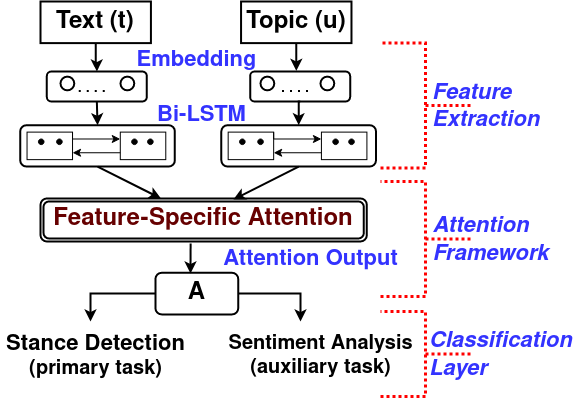
\includegraphics[width=0.85\linewidth]{images/shared_only_mark.png}
 % \includegraphics[scale=0.5]{architec.eps}
  %\setlength{\abovecaptionskip}{-0.3pt}
  %\setlength{\belowcaptionskip}{-15pt}
  \caption{Architectural diagram of the Shared-Only Multi-Task (SO-MT) Framework.}
  \label{shared_only}
  \vspace{-0.3cm}
\end{figure}
\begin{comment}
\begin{figure}
\centering
\includegraphics[width=1.05\linewidth]{images/main_rev_1.png}
 % \includegraphics[scale=0.5]{architec.eps}
  %\setlength{\abovecaptionskip}{-0.3pt}
  %\setlength{\belowcaptionskip}{-15pt}
  \caption{Architecture of the Shared-Private Multi-Task \\  (SP-MT) Framework }
  \label{sp_mt}
  \vspace{-0.5cm}
\end{figure}

\begin{figure}
\centering
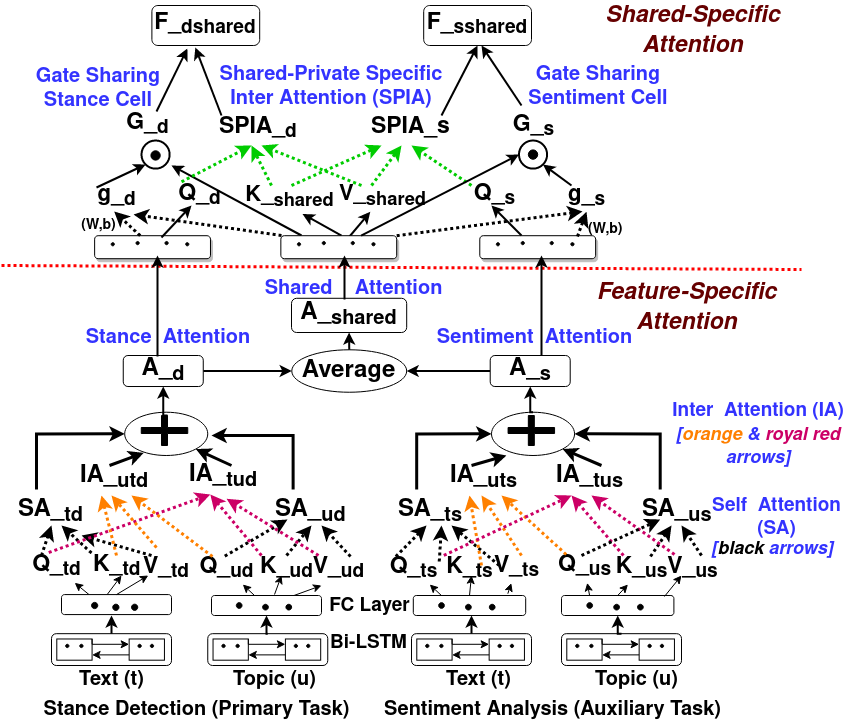
\includegraphics[width=1.1\linewidth]{images/attn_mark_rev.png}
 % \includegraphics[scale=0.5]{architec.eps}
  %\setlength{\abovecaptionskip}{-0.3pt}
  %\setlength{\belowcaptionskip}{-15pt}
  \caption{Architecture of the Shared-Private Multi-Task \\  (SP-MT) Framework }
  \label{sp_mt}
  \vspace{-0.5cm}
\end{figure}
\end{comment}

\begin{figure*}
\begin{minipage}{.5\linewidth}
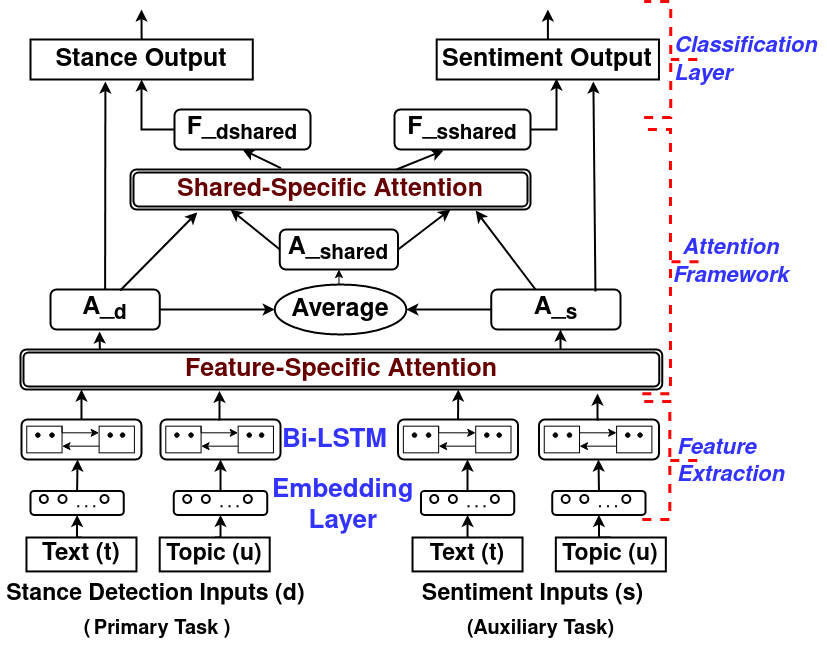
\includegraphics[width=1.02\linewidth]{images/main_rev_1_update.png}
 % \includegraphics[scale=0.5]{architec.eps}
  %\setlength{\abovecaptionskip}{-0.3pt}
  %\setlength{\belowcaptionskip}{-15pt}
  \caption{Architecture of the Shared-Private Multi-Task \\  (SP-MT) Framework }
  \label{sp_mt}
  \vspace{-0.5cm}
\end{minipage}
\begin{minipage}{.5\linewidth}
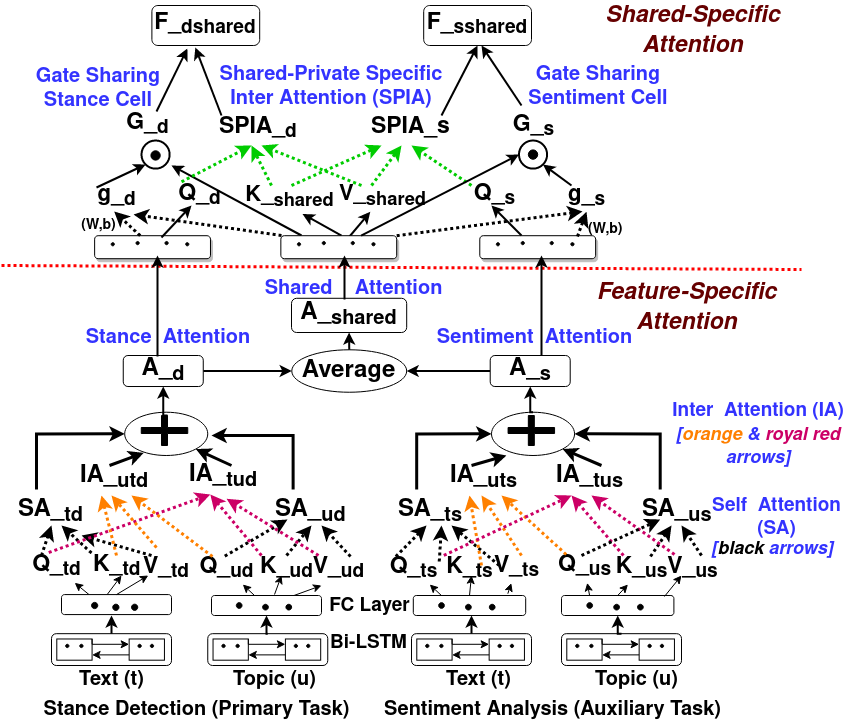
\includegraphics[width=1.05\linewidth]{images/attn_mark_rev.png}
 % \includegraphics[scale=0.5]{architec.eps}
  %\setlength{\abovecaptionskip}{-0.3pt}
  %\setlength{\belowcaptionskip}{-15pt}
  \caption{Attention Framework : (Top) Shared-Specific Attention; (Bottom) Feature-Specific Attention}
  \label{attn_frame}
  \vspace{-0.4cm}
\end{minipage}
\end{figure*}

\subsection{Components of the Model}\label{modelComp}
\subsubsection{Feature Extraction\\} 
\par\noindent {\textbf{Text}} : Each tweet text `T' contains $n_t$ number of words, where the embedding of each word $w_1,. . ., w_{n_{t}}$ is acquired from BERT \cite{DBLP:conf/naacl/DevlinCLT19} with dimension(d) = 768. We obtain final embedding for each tweet text as $T \in \mathbb{R}^{n_{t} \times d} $. Since Bi-LSTM has shown excellent performance in text classification due to its ability to learn long-term dependencies and incorporate past and future context information without retaining duplicate information \cite{DBLP:conf/coling/ZhouQZXBX16}, we use Bi-LSTM to sequentially encode the embedded input text representations. The embedded text is fed to Bi-LSTM with dimension $d_l$, which learns the long-term context dependent semantic features into hidden states. The final hidden matrix of text is $H_t \in \mathbb{R}^{n_{t} \times 2d_l} $. 
%\comMF{Please, make the text clearer, explain why we ended up with $2d_l$. You also could report some of this dimension in figure so that it is crystal clear the input dimension of the architecture}.  \comAU{Since it is bi-directional, therefore we end up with $2d_l$, i feel it will work and we have specify all the dimensions in section 5.2 Set-up. Please let me know should i mention here, or the in set up section only.}
\par\noindent {\textbf{Topic}} : Each tweet is tagged with the number of m-most similar topics based on the probability score assigned to each of the topics, where each topic is represented by the top `p' topic words created using BERTopic (described in section \ref{data_preprocess}). Here we represent the topic feature as `U' containing a set of $n_u$ words ($n_u$ $\le m\times p$), where the representation of each word $w_1,..., w_{n_{u}}$ are obtained from BERT with $d=768$. We obtain final embedding for each tweet topic as $U \in \mathbb{R}^{n_{u} \times d} $. This representation of topic is then fed to the Bi-LSTM layer with $d_l$ that sequentially encodes these representation, and gives the final hidden matrix of topic $H_u \in \mathbb{R}^{n_{u} \times 2d_l} $.

 
\subsubsection{Attention Framework} \label{attn_section}
%\comMF{Please, check once again and in case rephrase the entire section with better reference to the figure, for a fresh reader it is hard to find the subcomponent in the figure since they neither do not show the same name nor there is not clear refrence when tehy are constituted by several submodules}
%We apply attention framework similar to the \cite{vaswani2017attention}, where authors considered an attention function as a mapping on a set of queries, keys and values. In order to achieve queries, keys and values for the final modality representations, we pass the hidden matrix output from the Bi-LSTM layer of text($H_t$) and topic($H_u$) each through three fully connected layers with dimension $d_a$. There is a set of two triplets of query, key and value, for text($Q_t,K_t,V_t$) and topic($Q_u,K_u,V_u$) in SO-MT model while, we have a total of four triplets for SP-MT model, thus forming two pairs of two triplets each of text and topic belonging to each of the polarisation ( ($Q_{tp},K_{tp},V_{tp}$),($Q_{up},K_{up},V_{up}$) ), and sentiment ( ($Q_{ts},K_{ts},V_{ts}$),($Q_{us},K_{us},V_{us}$) ) tasks. Fig. \ref{attn_frame} visually shows how different queries, keys, and values are encoded to obtain different attention representations. Next, we describe the different attention mechanisms used for the proposed model : 
Attention mechanism has been used as an important component across a wide range of NLP models \cite{bahdanau2014neural}. Typically, the attention layer concentrates on the relevant part of the input and extracts the most important information from the input. We apply the attention framework similar to \cite{vaswani2017attention}, in which the authors consider an attention function as a mapping to a set of queries, keys, and values. To obtain queries, keys, and values for the final feature representations, we pass the hidden matrix output from the Bi-LSTM layer of text ($H_t$) and topic ($H_u$), respectively, through three fully connected layers of dimension $d_a$. There are two triplets of query, key, and value for text ($Q_t,K_t,V_t$) and topic ($Q_u,K_u,V_u$) in the model SO-MT, while we have a total of four triplets for the model SP-MT, forming two pairs of two triplets each for text and topic, which are used for stance detection (($Q_{td},K_{td},V_{td}$),($Q_{ud},K_{ud},V_{ud}$)) and sentiment (($Q_{ts},K_{ts},V_{ts}$),($Q_{us},K_{us},V_{us}$)) tasks respectively. Fig. \ref{attn_frame} visually shows the two attention frameworks used in our model: \textit{feature-specific attention} and \textit{shared-specific attention}. The lower part of the figure shows how different queries, keys, and values are encoded to obtain self-attention and inter-attention, which form the two sub-modules of feature-specific attention. The upper part of the figure shows the connections between queries, keys, and values to achieve shared-specific attention. In the following, we describe in detail the attention mechanisms used in our study.
\par \noindent \textbf{Feature-Specific Attention}\label{mod_section} We apply two types of attention to the features to capture the most informative parts of them. Fig. \ref{attn_frame} (bottom) shows the visual representation and connections of feature-specific attention. Feature-specific attention is further divided into Self Attention (SA) and Inter Attention (IA). %\comMF{for a fresh reader, it is difficult to identify what to look at the bottom-right of the figure. Think about a better referencing or some dashed box in figure with text label}. 

\par \noindent \textbf{\textit{Self Attention (SA)}} We use Self Attention (SA) to relate different positions of a single sequence of say tweet text or topic to quantify the most important part of that sequence \cite{vaswani2017attention}.  %, to capture the relation between current part and the previous part of the tweet text or topic.i.e. for every individual modality. SA is computed to relate different positions of a single sequence of say text or topic modality to quantify the most important part of that sequence \cite{NIPS2017_3f5ee243}.
% \vspace{-0.30cm}
\begin{gather}\label{eqn1}
        SA_j = softmax(Q_{j}K^T_{j})V_{j}
\end{gather}
% \setlength{\abovedisplayskip}{-1cm}
% \setlength{\belowdisplayskip}{-2cm}
% \vspace{-0.51cm}
\par \noindent SA scores are calculated using the equation \ref{eqn1}, where $SA_t \in \mathbb{R}^{n_{t} \times d_a} $, and $SA_u \in \mathbb{R}^{n_{u} \times d_a} $. Here, two SA scores are computed for SO-MT, while four such SA scores are required for SP-MT model ($SA_{td}, SA_{ud}, SA_{ts},SA_{us}$) (as shown with black dotted arrow connections in Fig. \ref{attn_frame} (bottom).

\par \noindent \textbf{\textit{Inter Attention (IA)}} We find out the Inter Attention (IA) scores to learn the interdependence between different features. IA scores are determined using below equations where query of one feature is intervened with key and value of the other. IA scores help to reveal the significant contributions amongst different inputs to learn optimal features for both tasks. The equations that represent the IA scores for text and topic ($IA_{tu}$, $IA_{ut}$) are:
%\vspace{-0.75cm}
\begin{gather}
    IA_{tu} = softmax(Q_{t}K^T_{u})V_{u}, \label{ia_1} \\
    IA_{ut} = softmax(Q_{u}K^T_{t})V_{t}, \label{ia_2}
\end{gather}
where $IA_{tu} \in \mathbb{R}^{n_{t} \times d_a} $, and $IA_{ut} \in \mathbb{R}^{n_{u} \times d_a} $. IA equations are represented graphically with orange and royal red dotted arrows in Fig. \ref{attn_frame} (bottom) part. The SA and IA scores are then concatenated finally, where A is directly used for shared-only (SO) variant (refer Fig. \ref{shared_only}) while average of attention vector ($A_{shared}$) specific to stance and sentiment tasks ($A_d$,$A_s$) is used for Shared-private (SP) variant of model (mentioned in Fig. \ref{attn_frame} (bottom)). 
\begin{gather}
    A    = concat(SA_{t},SA_u, IA_{tu},IA_{ut}), \\
    A_{d} = concat(SA_{td},SA_{ud}, IA_{tud},IA_{utd})), \label{attn_pol}\\
    A_{s} = concat(SA_{ts},SA_{us}, IA_{tus},IA_{uts})),\\
    A_{shared} = Average(A_{d},A_{s}) \label{attn_sh}
\end{gather}

\par \noindent \textbf{Shared-Specific Attention}\label{sharedattn_section} Some of the works mentioned in section \ref{rw_sent} focused on the orthogonal relationship between sentiment and stance detection. Although climate change deniers and proponents dominate in sentiment, there are a few examples where sentiment does not match attitude/stance (see Table \ref{tab:data1}). \cite{wu2019different} also mentioned the disadvantage of the shared-private model of multi-task learning, explaining that the shared space usually mixes some task-relevant features, which makes learning different tasks difficult. %Through the introduction of noise. 
To solve the above problems, we use the \cite{wu2019different} inspired shared-specific attention, which filters out the useless features that interfere with the model prediction and only pay attention to the selected features from the shared layer that lead to the correct predictions of the SP-MT model (see Fig. \ref{sp_mt}). Next, we describe the sub-modules to achieve the desired result (as shown in Fig. \ref{attn_frame} (top))
%Some of the works mentioned in section \ref{rw_pol} focused on the orthogonal relationship between sentiment and stance detection. Although, climate change deniers and believers have dominating sentiments, yet there are presence of few samples where sentiments are not in agreement with the stance(refer table \ref{tab:data1}). \cite{wu2019different} also mentioned the drawback of the shared-private model of multi-task learning, stating that the shared space usually mixes some task-relevant features, which makes the learning of different tasks difficult. %by introducing noise. 
%To tackle the above issues, we use shared specific attention inspired by the authors \cite{wu2019different}, that filters the useless features %that interfere with the model prediction
%,and provide attention to the selected features only from the shared layer that would lead to the correct predictions of the SP-MT model (shown in Fig. \ref{sp_mt}). Next, we describe the sub-modules to achieve the desired outcome (as shown in Fig. \ref{attn_frame} (upper)).

\par \noindent \textbf{\textit{Gate Sharing Cell}} We use similar approach used by authors \cite{wu2019different} where a single gate mechanism removes the useless shared features from shared layer. We first express the cell with reference to stance detection task. The stance specific, and shared attention scores ($A_d, A_{shared})$ from equations (\ref{attn_pol},\ref{attn_sh}) are passed through dense layers with $d_s$ units. The weights and biases are captured when passing $A_d$ through dense layer which are used for $A_{shared}$, and is expressed as gated sharing cell. %The cell is expressed with the equations :
\begin{eqnarray}
     g_d = \sigma(W_d . A_{shared}  + b_d)
    \label{eq:lstm}
\end{eqnarray}
where, $W_{d} \in \mathbb{R}^{n_{t}(d_s) \times n_{t}(d_s)} $ and $b_{d} \in \mathbb{R}^{1 \times n_{t}(d_s)} $. Similar equations are followed for sentiment task also, hence, we do not iterate here.
The final output of the shared features for both the task after filtering will be represented as :
\begin{gather}
    G_d    = g_d \odot A_{shared}, \\
    G_s    = g_s \odot A_{shared}
\end{gather}
where $\odot$ denotes element-wise multiplication. Fig. \ref{attn_frame} (top) shows the connections of gate sharing cell for stance detection and sentiment tasks.
\par \noindent \textbf{\textit{Shared-Private specific Inter Attention (SPIA)}} We use similar concept of the inter attention of feature-specific attention (equations \ref{ia_1}, \ref{ia_2}). We capture the important shared features relevant to the specific task, by using query matrix of the particular task (stance/sentiment) and keys and values of the shared task. The attention vectors ($A_d,A_s$) are passed through fully connected layers with $d_s$ units to create %query values 
$Q_d,Q_s$ for stance and sentiment tasks, while $A_{shared}$ is passed through dense layer to generate $K_{shared}$, and $V_{shared}$. %key and value for the shared task ($K_{shared},V_{shared}$). 
The equations are represented visually with green dotted arrows in Fig. \ref{attn_frame} (top) part.
\begin{gather}
    SPIA_{d} = softmax(Q_{d}K^T_{shared})V_{shared}, \\
    SPIA_{s} = softmax(Q_{s}K^T_{shared})V_{shared}
\end{gather}

\par \noindent \textbf{\textit{Fusion}} The final output of the shared layer is the fusion of the output of the gated cell and shared-private specific inter attention. Recently, fusion technique with absolute difference and element-wise product is found to be effective in \cite{mou2015natural}.
\begin{gather}
    C_1=[G_d;SPIA_d;G_d - SPIA_d;G_d \odot SSIA_d];\\
    C_2=[G_s;SPIA_s;G_s - SPIA_s;G_s \odot SSIA_s];\\
    F_{dshared} = \tanh(W_{fd}.C_1  + b_{fd}), \\
    F_{sshared} = \tanh(W_{fs}.C_2  + b_{fs})
\end{gather}

\subsubsection{Classification Layer} 
The final representation of the tweet obtained($A_d$,$A_s$) is passed through separate outputs for stance and sentiment tasks (for SO-MT model (Fig. \ref{shared_only}) ), however individual task specific tweet representations along with the shared layer representations are passed through two output channels, subjected to polarisation ($A_d$,$F_{dshared}$) and sentiment ($A_s$,$F_{sshared}$) tasks for SP-MT Model (Fig. \ref{sp_mt}). The task specific and shared loss are used as 
\begin{gather}
     L_{total} = L_{task} + \lambda L_{shared}
\end{gather}
where $\lambda$ = $0.5$ is a hyper-parameter \cite{DBLP:conf/acl/LiuQH17}.

\section{Experiment}
\subsection{Datasets} We evaluate our model performance and compare with the other baselines on the two datasets:

\par\noindent\textbf{Climate Change Data} The details of the data collection and statistics are covered in section \ref{dataset} and  table \ref{tab:data}.
\par\noindent\textbf{SemEval} is provided in the SemEval-2016 shared task 6.A on tweet stance detection \cite{mohammad2016semeval}. Each tweet is in favor, against or neutral corresponding to  one of the five targets: \textit{Atheism, Climate Change is a Real Concern, Feminist Movement, Hillary Clinton, and Legalization of Abortion(Abortion)}. There has been several works that use this benchmark dataset for stance classification.
\begin{table*}[]
\centering
\scalebox{0.75}{
\begin{tabular}{|c|c|c|c|c|c|c|c|c|}
\hline
\multirow{2}{*}{\textbf{Model}} &\multicolumn{4}{c|}{\textbf{Single-Task Stance Detection}} &\multicolumn{4}{c|}{\textbf{Single-Task Sentiment}}\\ 
\cline{2-9}
 &\multicolumn{2}{c|}{\textbf{Text}} &\multicolumn{2}{c|}{\textbf{Text+Topic}} &\multicolumn{2}{c|}{\textbf{Text}} &\multicolumn{2}{c|}{\textbf{Text+Topic}} \\ \cline{2-9} 
 &\textbf{Acc.} & \textbf{F1} & \textbf{Acc.} & \textbf{F1} & \textbf{Acc.} & \textbf{F1} & \textbf{Acc.} & \textbf{F1}\\ \hline
Shared-only (SO) &76.73$\pm$2.48 &70.75$\pm$2.11 &79.56$\pm$1.10 &75.72 $\pm$1.08 &71.61$\pm$0.45 &70.11$\pm$0.79 &75.82$\pm$2.03 &74.63$\pm$2.41\\ \hline
SO + Self Attn. (SA)  &80.29$\pm$0.55 &74.24$\pm$0.31 &82.88$\pm$0.78 &77.56 $\pm$0.87 &73.49$\pm$0.92 &72.57$\pm$1.27 &77.68$\pm$1.27 &76.59$\pm$1.66\\ \hline
   SO + Inter Attn. (IA)&81.33$\pm$1.04 &73.35$\pm$1.41 &83.13$\pm$1.42 &76.04 $\pm$1.11 &73.68$\pm$3.20 &72.23$\pm$3.14 &77.93$\pm$2.01 &74.11$\pm$1.98\\ \hline
{\begin{tabular}[c]{@{}l@{}}   SO + SA + IA \\ (Feature-Specific Attn.)\end{tabular}} &82.15$\pm$0.05 &76.78$\pm$0.81 &\textbf{85.01$\pm$1.05} &\textbf{80.03 $\pm$2.42} &76.21$\pm$0.84 &74.95$\pm$1.02 &\textbf{80.81$\pm$1.29} &\textbf{79.28$\pm$1.44}\\ \hline
\end{tabular}
}
\caption{Results of the Single-Task Stance Detection and Sentiment tasks for various combinations}
\label{single-task}
\end{table*}
\begin{table*}[]

\centering
\scalebox{0.75}{
\begin{tabular}{|c|c|c|c|c|c|c|c|c|}
\hline
\multirow{4}{*}{\textbf{Model}} &\multicolumn{8}{c|}{\textbf{Multi-Task Stance Detection + Sentiment}}\\ 
\cline{2-9}
&\multicolumn{4}{c|}{\textbf{Stance Detection}} &\multicolumn{4}{c|}{\textbf{Sentiment}}\\ 
\cline{2-9}
 &\multicolumn{2}{c|}{\textbf{Text}} &\multicolumn{2}{c|}{\textbf{Text+Topic}} &\multicolumn{2}{c|}{\textbf{Text}} &\multicolumn{2}{c|}{\textbf{Text+Topic}} \\ \cline{2-9} 
 &\textbf{Acc.} & \textbf{F1} & \textbf{Acc.} & \textbf{F1} & \textbf{Acc.} & \textbf{F1} & \textbf{Acc.} & \textbf{F1}\\ \hline
Shared-only (SO) &81.16$\pm$1.89 &77.01$\pm$2.61 &84.86$\pm$1.13 &81.66 $\pm$3.28 &75.44$\pm$1.23 &74.40$\pm$1.75 &80.49$\pm$2.05 &79.19$\pm$2.8\\ \hline
Shared-Private (SP)&84.64$\pm$1.95 &81.53$\pm$2.55 &87.47$\pm$2.01 &84.24 $\pm$2.04 &77.93$\pm$2.09 &74.11$\pm$2.19 &85.28$\pm$0.91 &84.58$\pm$1.02\\ \hline
{\begin{tabular}[c]{@{}l@{}}Shared-Private (SP) +  \\ Feature-Specific Attn.\end{tabular}}  &86.49$\pm$2.29 &81.67$\pm$3.21 &91.31$\pm$1.06 &85.93 $\pm$1.22 &81.46$\pm$0.71 &80.71$\pm$0.39 &85.46$\pm$0.9 &84.73$\pm$1.10\\ \hline
{\begin{tabular}[c]{@{}l@{}}Shared-Private (SP) +  \\ Shared-Specific Attn.\end{tabular}}  &88.10$\pm$1.04 &84.09$\pm$1.39 &92.29$\pm$1.32 &86.12 $\pm$1.4 &81.67$\pm$0.61 &80.89$\pm$0.32 &87.59$\pm$0.45 &87.07$\pm$0.39\\ \hline
{\begin{tabular}[c]{@{}l@{}}Shared-Private +  \\ Feature-Sp. Attn. + \\ Shared-Sp. Attn. \\ (SP-MT) \end{tabular}}  &89.99$\pm$2.67 &86$\pm$2.02 &\textbf{93.95$\pm$1.27} &\textbf{90.24 $\pm$1.16} &84.60$\pm$0.44 &83.98$\pm$0.81 &\textbf{89.08$\pm$1.01} &\textbf{88.48$\pm$1.60}\\ \hline

\end{tabular}
}
\caption{Results of the Multi-Task Stance Detection and Sentiment tasks for various combinations}
\label{multi-task}
\end{table*}
\subsection{Set-up} We use the python-based library Keras\footnote{https://keras.io/} at various stages of our implementations. %We consider the accuracy and macro F1 scores from the stratified cross-validation experiments to evaluate the performance of our models. 
For the experiments, we perform stratified k-fold cross-validation on our dataset, oversample the minority class (deniers) in the k-1 training data using the sklearn resampling technique, and report the averaged scores and standard deviation (over 5 folds) for the accuracy and F1 scores. We select $m=5$ and $p=10$, which fits our dataset well, where $m$ denotes the number of most similar topics and each topic contains $p$ number of words for the topic feature of each tweet. In the feature extraction sub-module, Bi-LSTM ( $d_l$ ) with $100$ memory cells is used. The dimensions $d_a$ and $d_s$ of the fully connected layers used in the attention framework to extract queries, keys and values for feature-specific and shared-specific attention (refer section \ref{attn_section}) are used with $100$ units each. The stance and sentiment output channels contain $2$ and $3$ output neurons, respectively. The loss functions binary cross-entropy and categorical cross-entropy are used for the stance and sentiment output channels, respectively. The experiments are run on an NVIDIA GeForce GTX 1080Ti GPU and the models are optimized using Adam optimizer with a learning rate of $0.0001$. All these values are selected using TPE in the hyperopt python library \cite{bergstra2013hyperopt} and after a thorough sensitivity analysis of the parameters that minimise the loss functions.
%\comAU{will change as per final results.} We report all the results using k-fold cross validation technique. The complete climate change dataset is randomly divided into k equal sized subsamples, where a single subsample is retained as the validation data for testing, and the remaining k-1 subsamples are used as training data. Here, we use k=5 for cross validation. We select m-most similar topics, where each topic contains $p$ number of words for every tweet topic modality. We carefully select $m=5$, and $p=10$ \comMF{Are these parameters m and p only introduced here? In any case, it would be beneficial for the reader to report the full name for both parameters in terms of what they represent}. In feature extraction sub-module, Bi-LSTM ( $d_l$ ) with 100 memory cells are used. The dimension $d_a$, $d_s$ \comMF{I know you introduced that before, but as reminder, report the full name} are used with 100 units. The polarisation and sentiment output channel contain 2 and 3 output neurons respectively. The loss functions binary cross-entropy and categorical cross-entropy are used for polarisation and sentiment output channels. Adam optimizer with $0.0001$ learning rate are found to be optimum for the experiments. All these values are selected using TPE in Hyperopt python library, and after a thorough sensitivity analysis of the parameters that minimize the loss functions. 

\subsection{Baseline Techniques} \label{baselines_section}
We compare our proposed approach with the following baselines on our climate change dataset :
\par\noindent\textbf{Logistic regression \cite{argyris2021using}}: This study use logistic regression with Count Vectorizer feature extraction method to classify vaccine-related tweets into provaccine, antivaccine, and neutral stances.

\par\noindent\textbf{ESD \cite{vychegzhanin2021new}}: The authors form a relevant feature set using an ensemble of feature selection methods and propose the model ESD by selecting an optimal ensemble of classifiers. They evaluate the performance of the model using the UKP Sentential Argument Mining Corpus and the SemEval-2016 dataset.

\par\noindent\textbf{HAN \cite{wang2020neural}}: In this article, researchers proposed a hierarchical attention neural model, focusing on different features such as document, sentiment, dependency, and argument representations. They evaluated the model performance on SemEval-2016 and the H\&N14 dataset.

\par\noindent\textbf{AT-JSS-LEX \cite{li2019multi}}: is a multi-task framework for stance detection with sentiment analysis as auxiliary task. The attention mechanism of the model is guided by target-specific attention along with sentiment and stance lexicons. 

\par\noindent\textbf{MNB \cite{kabaghe66classifying}}: Multinomial naive bayes performed better with respect to other models proposed in the study, to classify tweets into positive, negative or neutral beliefs towards climate change.

\par\noindent\textbf{DNN \cite{chen2019detecting}}: Deep Neural Network (DNN) is used as a classifier to identify users who either believe or deny climate change based on the content of tweets. The model's performance is assessed on the real-time collection of climate change twitter data.
\par\noindent\textbf{SVM-ngram \cite{sobhani2016detecting}}: is trained on word and character n-grams features for stance detection task on SemEval 2016 dataset. The model surpassed the best model in SemEval-2016 competition.

\par\noindent We evaluate our model performance on \textit{SemEval 2016} dataset and contrast with the these state-of-the art models :  \textbf{ESD} \cite{vychegzhanin2021new}, \textbf{HAN} \cite{wang2020neural}, \textbf{AT-JSS-LEX} \cite{li2019multi}, and \textbf{SVM-ngram} \cite{sobhani2016detecting} as described above.



\section{Result and Analysis}
In this section, we investigate the performance of the proposed approach. We first compare different single-task and multi-task variants and then compare them with the state-of-the-art methods mentioned in section \ref{baselines_section}. We also analyze the importance of each feature and the different variants of the attention framework. We report all the results of the five-fold cross-validation (mean and standard deviation of accuracy and F1 score) for the different combinations of the proposed system.
\begin{table*}
\centering
\scalebox{0.85}{
% \resizebox{1.65\linewidth}{!}{
\begin{tabular}{|l|l|l|l|l|l|}
\hline
\textbf{No.}&\textbf{Tweet} &\textbf{Sentiment} & \textbf{True} & \textbf{{\begin{tabular}[c]{@{}l@{}}Predicted \\ Stance \end{tabular}}} & \textbf{{\begin{tabular}[c]{@{}l@{}}Predicted \\ Stance + \\ Sentiment \end{tabular}}} \\ \hline
1. &My family support Oil and Gas! ClimateHoax &positive  &denier &\color{red}believer &denier \\ \hline
2. &{\begin{tabular}[c]{@{}l@{}}Once again brainwashing kids to push the green tax agenda,\\ under the globalwarminghoax umbrella! Stop\end{tabular}} &negative  &denier &denier &denier \\ \hline
%2. &{\#ClimateHoax harms children. Time to drop the lie as hard as \#ToxicCRT. \#ProtectOurKids from \#GlobalistPricks} &negative  &denier &denier &denier \\ \hline
3. &His Green BS policies will send us back to the Dark Ages. ClimateChangeHoax &negative  &denier &\color{red}believer &denier \\ \hline
4. &{\begin{tabular}[c]{@{}l@{}}ClimateHoax The climate has fluctuated since the  time of creation,\\ and nothing those people will do can change that one way or the other\end{tabular}} &neutral  &denier &\color{red}believer &denier \\ \hline
5. &{\begin{tabular}[c]{@{}l@{}}And yet, there are those who deny climate change?? Ice-shelves breaking off,\\ heat waves, etc. Sad ScienceIsReal\end{tabular}} &negative  &believer &\color{red}denier &believer \\ \hline
6. &{\begin{tabular}[c]{@{}l@{}}Have you seen this? Its very moving. We definitely need more ClimateAction\end{tabular}} &positive  &believer &believer &believer \\ \hline
%6. &@UN Climate changes often depending on country you are in! \#Climatechangehoax climatechangehoax &neutral  &denier &\color{red}believer &\color{red}believer \\ \hline
7. &{\begin{tabular}[c]{@{}l@{}}For those adamant that global warming is real, THIS is Today in Alaska.\\ Four inches of snow overnight, and  still coming down! ClimateChange\end{tabular}} &neutral  &denier &\color{red}believer &\color{red}believer \\ \hline
%8. &{\begin{tabular}[c]{@{}l@{}}Thousands of people fly on their individual jets all around the world,\\ then drive in large, heavy, bulletproof, gas guzzling SUV..\#ClimateChangeHoax\end{tabular}} &neutral  &denier &\color{red}believer &\color{red}believer \\ \hline
%7. &{No such thing as climate change but yes I've noticed all the private jets and planes that are used by the governmen}  &neutral  &denier &\color{red}believer &\color{red}believer \\ \hline

%8. &{\begin{tabular}[c]{@{}l@{}}Shell says that oil companies are not welcome at COP26. But here we see\\ Biden's 85 car cavalcade practising in Rome. Doubt there are many EVs there...\end{tabular}} &neutral &denier &\color{red}believer &\color{red}believer \\ \hline

8. &{\begin{tabular}[c]{@{}l@{}}I am glad you went by plane. Way better for our climate instead of zoommeetings...\end{tabular}} &positive &believer &\color{red}denier &\color{red}denier \\ \hline

%10. &{\begin{tabular}[c]{@{}l@{}}They can't even predict the weather 48 hours in advance,\\ but they do know what the weather will be 30 years from now..\end{tabular}} &neutral &denier &\color{red}believer &\color{red}believer \\ \hline

9. &{\begin{tabular}[c]{@{}l@{}}Over 60 today. Over 6" of snow tomorrow. But yeah, climatechange is total bullshit right?\end{tabular}} &negative &believer &\color{red}denier &\color{red}denier \\ \hline

%12. &{\begin{tabular}[c]{@{}l@{}}I really wish people would stop calling climate change deniers "skeptics" and use \\something a little more accurate. Like "dumbasses," "mentally stunted potatoes,"\\ or "those possessing ulterior motives." #ClimateChangeIsReal\end{tabular}} &negative &believer &\color{red}denier &\color{red}denier \\ \hline

\end{tabular}

%}
}
 \setlength{\abovecaptionskip}{2pt}
  %\setlength{\belowcaptionskip}{-5pt}
\caption{Few example tweets with ground truth and predicted labels for single and multi-task models}
\label{examples}
\end{table*}
The Tables \ref{single-task} and \ref{multi-task} illustrate the results of the single-task and the various combinations of the proposed multi-task models for both the stance detection and sentiment tasks. It is evident that the addition of topic words consistently improves the performance of the models. This improvement means that the proposed architecture makes very effective use of the interaction between input features. This shows the importance of incorporating multiple features for various analysis tasks.

\subsection{Comparison amongst Single-Task and Multi-task Framework}
\par \noindent From the tables \ref{single-task} and \ref{multi-task}, the multi-task variants perform better than the single-task variants by achieving an average macro F1 score of $90.24$ and $88.48$ for the stance detection (primary) and sentiment analysis (auxiliary) tasks respectively. The results show that the sentiment and stance tasks improve each other's performance when learned together. The single stance detection task is able to correctly label some tweets from deniers and believer that contain predominantly negative and positive sentiments, respectively (examples $2$ and $6$ from Table \ref{examples}). However, examples $1$, $4$, and $5$ from Table \ref{examples} clearly show that the stance task, together with the sentiment analysis task, is able to unambiguously identify denier and believers tweets with the corresponding less dominant positive, neutral, and negative sentiment polarities. As stated earlier, we consider sentiment analysis as an auxiliary task that supports the main task, i.e., stance detection. However, we report the performance of the sentiment task for the proposed model for both single-task and multi-task frameworks in the tables \ref{single-task} and \ref{multi-task} to illustrate the impact of the main task on the auxiliary task and to show that the multiple features in the form of tweet text and topic words, as well as the attention framework, also benefit the sentiment classification task. However, we do not make explicit efforts to improve the model performance on the auxiliary task.
\begin{comment}
\begin{table}
\centering
\scalebox{0.60}{
\resizebox{1.65\linewidth}{!}{
\begin{tabular}{|l|l|l|l|l|l|}
\hline
\textbf{S.No.}&\textbf{Tweet} &\textbf{Sentiment} & \textbf{True} & \textbf{{\begin{tabular}[c]{@{}l@{}}Predicted\\ Polarisation \end{tabular}}} & \textbf{{\begin{tabular}[c]{@{}l@{}}Predicted\\ Polarisation \\+ Sentiment \end{tabular}}} \\ \hline
1. &My family support Oil and Gas! \#ClimateHoax  &positive  &denier &\color{red}believer &denier \\ \hline
2. &{\begin{tabular}[c]{@{}l@{}}Once again #brainwashing kids to push the #green \\ tax agenda, under the #globalwarminghoax umbrella! Stop\end{tabular}} &negative  &denier &denier &denier \\ \hline
%2. &{\#ClimateHoax harms children. Time to drop the lie as hard as \#ToxicCRT. \#ProtectOurKids from \#GlobalistPricks} &negative  &denier &denier &denier \\ \hline
3. &{\begin{tabular}[c]{@{}l@{}}His Green BS policies will send us back to the \\Dark Ages. ClimateChangeHoax\end{tabular}} &negative  &denier &\color{red}believer &denier \\ \hline
4. &{\begin{tabular}[c]{@{}l@{}}ClimateHoax The climate has fluctuated since the \\ time of creation, and nothing those people will \\ do can change that one way or the other\end{tabular}} &neutral  &denier &\color{red}believer &denier \\ \hline
5. &{\begin{tabular}[c]{@{}l@{}}And yet, there are those who deny climate change??\\ Ice-shelves breaking off, heat waves, etc. #Sad #ScienceIsReal\end{tabular}} &negative  &believer &\color{red}denier &believer \\ \hline
6. &{\begin{tabular}[c]{@{}l@{}}Have you seen this? Its very moving. We definitely \\need more #ClimateAction\end{tabular}} &positive  &believer &believer &believer \\ \hline
%6. &@UN Climate changes often depending on country you are in! \#Climatechangehoax climatechangehoax &neutral  &denier &\color{red}believer &\color{red}believer \\ \hline
7. &{\begin{tabular}[c]{@{}l@{}}For those adamant that global warming is real, \\THIS is Today in Alaska. Four inches of snow \\overnight, and still coming down! #ClimateChange\end{tabular}} &neutral  &denier &\color{red}believer &\color{red}believer \\ \hline
8. &{\begin{tabular}[c]{@{}l@{}}#ClimateChangeActivists Thousands of people fly on\\ their individual jets all around the world,\\ then drive in large, heavy, bulletproof, gas guzzling SUV\\ ...#ClimateChangeHoax\end{tabular}} &neutral  &denier &\color{red}believer &\color{red}believer \\ \hline
%7. &{No such thing as climate change but yes I've noticed all the private jets and planes that are used by the governmen}  &neutral  &denier &\color{red}believer &\color{red}believer \\ \hline
\end{tabular}

 }
}
 \setlength{\abovecaptionskip}{2pt}
  \setlength{\belowcaptionskip}{-10pt}
\caption{Few example tweets with ground truth and predicted labels for single task and multi task models}
\label{examples}
\end{table}
\end{comment}
%%% updation 


\begin{table}
\centering
\scalebox{0.70}{
\begin{tabular}{|l|l|l|}
\hline
\textbf{Model} &\textbf{Training Time (secs)} &\textbf{Mean Accuracy}  \\ \hline
{\begin{tabular}[c]{@{}l@{}} Single Task Best \\ (SO + SA + IA) [Table 5]\end{tabular}} &870 &85.01 \\ \cline{1-3}
\multicolumn{3}{|c|}{\textbf{Multi Task Variants} [Refer Table 6]} \\ \hline
Shared-only (SO) &918 &84.86 \\ \hline
Shared-Private (SP) &1218 &87.47 \\ \hline
{\begin{tabular}[c]{@{}l@{}}Shared-Private (SP) +  \\ Feature-Specific Attn.\end{tabular}} &1419 &91.31 \\ \hline
{\begin{tabular}[c]{@{}l@{}}Shared-Private (SP) +  \\ Shared-Specific Attn.\end{tabular}} &1506 &92.29 \\ \hline
{\begin{tabular}[c]{@{}l@{}}Shared-Private +  \\ Feature-Sp. Attn. + \\ Shared-Sp. Attn. (SP-MT) \end{tabular}} &1791 &93.95 \\ \hline
\end{tabular}
}
\caption{Training time of Different Text + Topic Models}
 \setlength{\abovecaptionskip}{2pt}
\label{tab_training}
\end{table}

\subsection{Comparison amongst Different Multi-task Frameworks} 
Table \ref{multi-task} shows the improvement of the multi-task framework from the shared-only variant (Fig. \ref{shared_only}) to the shared-private multi-task model(SP-MT) (Fig. \ref{sp_mt}). The inclusion of feature-specific and shared-specific attention frameworks helped the multi-task models focus on the important parts of the features and effectively discard the useless shared features, resulting in a $7.40\%$ increase in accuracy and a $12.46\%$ increase in F1 score. Furthermore, in Table \ref{tab_training} we give the training times of the best performing single-task model and different variants of the multi-task model for 20 epochs to analyze the additional time required by the best performing multi-task model with text and topic as input features (SP-MT) compared to other variants. As can be seen from the table \ref{tab_training}, SP-MT requires about $15$ more minutes (approximately twice the time) to achieve a $10.51$\% improvement in accuracy compared to the best performing single-task model, while SP-MT requires $9.5$ more minutes to achieve a $7.4$\% improvement in performance compared to the shared-private multi-task variant.
\par \noindent All results reported here are statistically significant as we performed a t-test at the $5\%$ significance level \cite{welch1947generalization} against the null hypothesis, which states that the mean accuracy/F1 score of all the multi-task variants is more when compared to the the best performing proposed model SP-MT (Shared-Private + Feature-Specific Attention +Shared-Specific Attention) [refer table \ref{multi-task}]. If the p-value is significant ($p<0.05$), we reject the null hypothesis. Our best performing proposed model outperforms all the other multi-task variants while meeting statistical significance under t-tests ($p<0.05$). For the confidence analysis, we also report the p-values and t-test statistics of all the multi-task variant models compared to the best performing model in tables $1$ and $2$ in Supplementary.
%\textbf{AU: need to create tables in supplementary}}
\subsection{Comparison with the Baseline Methods}
In Table \ref{baselines}, we report the results for the baseline methods by re-implementing them on the Climate Change dataset (section \ref{dataset}). It is observed that our proposed multi-task approach SP-MT outperforms the SOTA approaches in terms of accuracy and F1 score. Our best performing model achieved better results compared to ESD \cite{vychegzhanin2021new} and HAN \cite{wang2020neural}. This highlights that the shared-private multi-tasking approach takes advantage of task-specific and invariant features to improve classification task performance. Although the AT-JSS-LEX \cite{li2019multi} model was implemented with a multi-tasking approach, our model performs better because it keeps the task-dependent and task-independent feature spaces separate and removes the useless shared features that hinder task performance of the stance detection, demonstrating the importance of the shared-specific attention framework. It is also observed that the methods that use sentiment features (ESD, HAN, and AT-JSS-LEX) perform better than the other baselines. This proves the importance of the proposed sentiment analysis approach for climate change. Our best performing single-task polarization framework (Table \ref{single-task}) also outperforms MNB, DNN, and SVM-ngram approaches. This justifies the benefits of using topic words in addition to tweet text and feature-specific attention framework to improve the performance of the model. \\
\noindent Consequently, we also performed a comparative analysis of the proposed multi-tasking approach SP-MT with the state-of-the-art models (SOTA) on the SemEval 2016 dataset. The model is trained with three polarized classes \textit{(Favour, Against, None)} and the metrics ($F_{avg}$, $MacF_{avg}$) are evaluated according to the procedure defined in \cite{li2019multi}. Table \ref{sem_eval} shows that our approach outperforms other methods with an overall $MacF_{avg}$ value of $66.84$. Our proposed framework performs better in the climate, feminism, and abortion domains, while the $F_{avg}$ values are comparable in the atheism and Hillary domains, showing that our framework generalises well in different domains.

\begin{comment}
\begin{table}
\centering
\scalebox{1}{
\resizebox{1\linewidth}{!}{
\begin{tabular}{|c|c|c|c|c|c|c|c|c|}
\hline
\multirow{4}{*}{\textbf{Model}} &\multicolumn{8}{c|}{\textbf{Multi Task Polarisation + Sentiment}}\\ 
\cline{2-9}
&\multicolumn{4}{c|}{\textbf{Polarisation}} &\multicolumn{4}{c|}{\textbf{Sentiment}}\\ 
\cline{2-9}
 &\multicolumn{2}{c|}{\textbf{Text}} &\multicolumn{2}{c|}{\textbf{Text+Topic}} &\multicolumn{2}{c|}{\textbf{Text}} &\multicolumn{2}{c|}{\textbf{Text+Topic}} \\ \cline{2-9} 
 &\textbf{Acc.} & \textbf{F1} & \textbf{Acc.} & \textbf{F1} & \textbf{Acc.} & \textbf{F1} & \textbf{Acc.} & \textbf{F1}\\ \hline
Shared-only (SO) &2.61E-07 &1.54E-06 &1.20E-05 &3.29E-05 &3.72E-07 &1.20E-05 &0.00017 &9.94E-06\\ \hline

Shared-Private (SP)&1.24E-06 &0.0023 &9.70E-06 &0.00036 &0.0014 &0.00015 &0.0027 &5.05E-05\\ \hline
{\begin{tabular}[c]{@{}l@{}}Shared-Private (SP) +  \\ Modality Specific Attn.\end{tabular}}  &0.00029 &0.00023 &0.0084 &0.00061 &1.94E-06 &1.87E-05 &0.0017 &0.00051 \\ \hline

{\begin{tabular}[c]{@{}l@{}}Shared-Private (SP) +  \\ Shared-Specific Attn.\end{tabular}}  &2.34E-05 &0.0077 &0.0021 &0.0014 &4.57E-06 &6.16E-06 &0.007 &0.00836\\ \hline
\end{tabular}
}
}
\caption{p-values of all the multi task variant models compared to the best performing SP-MT (Shared-Private + Feature-Sp. Attn + Shared-Sp. Attn)}
\label{pvalues}
\end{table}

\end{comment}


\subsection{{Error Analysis}} \label{Error_analysis}
%We conduct a in-depth error analysis to understand where the proposed model faltered. These are the following scenarios : (i). The climate change dataset has a imbalanced dataset with high proportion of believer tweets and an imbalance ratio of 1:6 for denier to believer category, resulting in low f1-scores when compared with the accuracy. (ii) The sample tweets 7 and 8 from table \ref{examples} shows the incorrect predictions by both the single task and multi task proposed models. These both examples contain a pinch of sarcasm attached to the tweet text where tweet authors sarcastically expressed their notions of climate change denial with sarcasm. In example 7, the denier tweet contains the words such as \textit{real, snow overnight} are mostly occurred with the believer tweets confuse the model and result in the wrong prediction. Similarly, there is a mixture of believer and denier statements in the tweet sample 8 with the hidden sarcasm leading to the incorrect prediction label. To counter these, there is a need to investigate the role of sarcasm and aspect-based sentiment that could further improve the model performance.
We perform an in-depth error analysis to understand where the proposed model has faltered. These are the following scenarios: \textbf{(i)} The climate change dataset is an imbalanced dataset with a high proportion of believer tweets, resulting in low F1 values compared to accuracy. Although we applied oversampling to partially counter this problem, even finer categories of believers can be identified and labeled, which can be beneficial for the model to learn different classes with a clear separation of distribution in tweets, such as ``tweet conveys causes of climate change'' or ``tweet believes in human-caused climate change''. \textbf{(ii)} We determine the frequency of unigrams and bigrams extracted using TF-IDF and find that some of the denier's tweets containing either rarely used keywords or keywords frequently used in believers' tweets were misclassified. For example, the denier's tweet in example $7$ (table 7) contains words such as \textit{real, snow overnight}, which are most commonly found in believers' tweets and confuse the model and lead to an incorrect prediction. \textbf{(iii)} We investigated that of the total misclassified denier tweets, $35.7\%$ of the tweets contained sarcasm to express their denial. Of the sarcastic denier tweets, $50.16\%$ of the tweets have positive sentiment, $31.70\%$ have neutral sentiment, and the rest have negative sentiment, while $25.78\%$ of the misclassified believer tweets have sarcastic labels (examples $8$ and $9$ of table 7). The labeling of sarcasm is based on the majority vote of three trained annotators with an inter-rater agreement of $0.78$, calculated with the Fleiss-Kappa measure. This motivated us to investigate the presence of sarcasm in climate change tweets to further improve the performance of the model as a part of our future work. %Sample tweets 7 and 8 from Table \ref{examples} show the flawed predictions of both the proposed single task and multi task models. These two examples contain a pinch of sarcasm in the text of the tweet, in which the authors of the tweet use sarcasm to express their ideas about climate change denial.  Similarly, with a mixture of believer and denier statements in tweet example 8, the hidden sarcasm leads to a false prediction. To counter this, it is necessary to investigate the role of sarcasm and aspect-based sentiment to further . 
\begin{table}
\centering
\scalebox{0.67}{
% \resizebox{1\linewidth}{!}{
\begin{tabular}{|c|c|c|}
\hline
\textbf{Model} &\textbf{Accuracy} &\textbf{F1-score} \\ \hline
Proposed SP-MT (Fig. \ref{sp_mt}) &\textbf{93.95} &\textbf{90.24} \\ \hline
LR (Argyris et al. 2021) &81.48 &81.00 \\ \hline
ESD \cite{vychegzhanin2021new} &89.65 &85.11 \\ \hline
HAN \cite{wang2020neural} &89.47 &86.00 \\ \hline
AT-JSS-LEX \cite{li2019multi} &88.02 &84.01 \\ \hline
MNB \cite{kabaghe66classifying} &85.44 &78.08 \\ \hline
DNN \cite{chen2019detecting} &84.61 &76.23 \\ \hline
SVM-ngram \cite{sobhani2016detecting} &85.55 &66.33 \\ \hline
\end{tabular}

%  }
}
 \setlength{\abovecaptionskip}{2pt}
  \setlength{\belowcaptionskip}{-6pt}
\caption{Results of Proposed Framework SP-MT with baselines on our Climate Change Dataset}
\label{baselines}
\end{table}

\begin{table}
\centering
\scalebox{0.61}{
% \resizebox{1\linewidth}{!}{
\begin{tabular}{|c|c|c|c|c|c|c|}
\hline
\textbf{Model} &\textbf{{\begin{tabular}[c]{@{}l@{}}Atheism\\ $F_{avg}$ \end{tabular}}} &\textbf{{\begin{tabular}[c]{@{}l@{}}Climate\\ $F_{avg}$ \end{tabular}}} &\textbf{{\begin{tabular}[c]{@{}l@{}}Feminism\\ $F_{avg}$ \end{tabular}}} &\textbf{{\begin{tabular}[c]{@{}l@{}}Hillary\\ $F_{avg}$ \end{tabular}}} &\textbf{{\begin{tabular}[c]{@{}l@{}}Abortion\\ $F_{avg}$ \end{tabular}}} &Mac $F_{avg}$ \\ \hline
Proposed SP-MT(Fig.\ref{sp_mt}) &69.5 &\textbf{63.5} &\textbf{63.2} &67.5 &\textbf{70.5} &\textbf{66.84} \\ \hline
{{\begin{tabular}[c]{@{}l@{}}ESD \\ (Vychegzhanin and\\ Kotelnikov 2021) \end{tabular}}} &66.64 &43.82 &62.85 &67.79 &64.94 &61.20 \\ \hline
HAN \cite{wang2020neural} &\textbf{70.53} &49.56 &57.50 &61.23 &66.16 &61.00 \\ \hline
{{\begin{tabular}[c]{@{}l@{}}AT-JSS-LEX\\ \cite{li2019multi}\end{tabular}}} &69.22 &59.18 &61.49 &\textbf{68.33} &68.41 &65.33 \\ \hline
{{\begin{tabular}[c]{@{}l@{}}SVM-ngram\\(Sobhani,  Mohammad,\\  and  Kiritchenko2016) \end{tabular}}}  &65.19 &42.35 &57.46 &58.63 &66.42 &58.01 \\ \hline
\end{tabular}
}
 \setlength{\abovecaptionskip}{2pt}
  %\setlength{\belowcaptionskip}{-10pt}
\caption{Results of Proposed Framework SP-MT with baselines on SemEval 2016 Dataset}
\label{sem_eval}
\end{table}

\section{Privacy and Ethics}
Although social media offers innovative ways to raise awareness about climate change, phenomena such as climate denial and climate delay have become a serious problem for scientists and the government to convince people of the importance of understanding the current climate crisis. Climate change deniers are not only skeptical about climate change but also emphasize the disadvantages of all measures proposed to combat climate change and abandon the idea that it is not possible to prevent climate change. This often leads to the spread of misinformation, resulting in a delay in the implementation of effective climate change mitigation measures \cite{zhou2021confirmation}. Since our work is dedicated to classifying Twitter content into climate change deniers or believers, the proposed approach can be useful for government agencies, researchers, and tech companies that monitor such content on social media to identify and intervene tweets from climate change deniers. The proposed approach is useful in combating climate misinformation by identifying posts by climate change deniers and reducing the spread of such content that is deemed false or misleading.
\par \noindent The input feature of the proposed model, such as the tweet text, is available as soon as the user posts something. However, the topic feature can be extracted by performing topic modeling for a collection of tweets after a fixed interval, e.g., after every 5, 10, 15, or t minutes of duration. Therefore, our proposed approach can be used in a real-time environment by interested agencies and authorities to classify social media content into one of the two polarized classes.
\par \noindent Although we conduct our work with public data from social media, however, we are committed to protecting the privacy of individuals and therefore avoid providing personally identifiable content. The dataset that is made publicly available consists only of tweet IDs and comments.

\section{{Conclusion and Future Work}}
%In this work, we studied the role of sentiment in classification of polarised stances of climate change Twitter data. We curate a novel dataset, that contains annotations for both polarisation and sentiment analysis task. We propose a Shated-Private Multi-task framework  for joint optimization ofpolarisation and sentiment analysis. The propsoed module employs modality specific and shared specific attention to fuse multiple modalities and learn useful and relevant private and shared features across all the tasks. Results show that multi-modality and multi-tasking boosted the performance of polarisation task compared to its uni-modal and single task variants.
%In future, attempts will be made to analyze what other aspects of natural language such as sarcasm detection, aspect based sentiment and emotion recognition might assist in the classification of polarised climate change stances with more precision.
In this paper, we focus on the importance of classifying Twitter content into climate change deniers and believers, because climate change deniers emphasize the downsides of any action to address climate change, which often leads to the spread of misinformation and delays the implementation of effective action to mitigate climate change. Our proposed approach, implemented in real-time, can be useful for government agencies, researchers, and tech companies in combating climate misinformation by identifying content that denies climate change and reducing the spread of such posts that are considered misleading. \\
\noindent In this work, we investigated the role of sentiment in classifying stance of the tweets related to climate change. We curate a novel dataset that includes annotations for both stance detection and sentiment analysis tasks, which will be useful to the research community in exploring other needed classification tasks. We propose a shared-private multi-task framework for the optimization of stance detection task benefiting from the sentiment analysis (auxiliary task). The proposed module uses feature-specific and shared-specific attention to fuse multiple features and learn useful and relevant private and shared features for both tasks. The results show that multi-tasking increased the performance of the stance detection task compared to its uni-modal and single-task variants. Although we examined the performance of the proposed approach in detecting attitudes in the domain of climate change, the performance of the model on the SemEval dataset shows that it is much more broadly applicable beyond the domain of climate change, suggesting that our framework can generalize well in different domains.
Future work will attempt to analyse what other aspects of natural language, such as sarcasm, aspect-based sentiment, and emotion recognition, might help to more accurately classify  attitudes toward climate change. The inclusion of other modality encodings such as images, emoji, and advanced architectures will also be the subject of our future work.

%Although social media sites provide innovative opportunities for spreading awareness about climate change, phenomena such as climate denial and climate delay have emerged as a serious problem for the scientists and government to make people believe the importance of understanding the ongoing climate crisis. Climate change deniers are not only skeptic about climate change but also emphasize the downside of any actions proposed to tackle climate change and surrendering the idea that it is not possible to prevent climate change, often resulting in spreading misinformation which leads to delay in implementing effective mitigation measures. Since, our work is dedicated to classify stances of the twitter content into climate change denier or believer, the proposed approach can be beneficial to government agencies, researchers and tech companies that might monitor such content on social media to identify climate change deniers tweets and intervene. The proposed approach can be useful to combat climate misinformation by identifying the climate change denier posts and reducing the distribution of such rated false or misleading content. \par\noindent Although our work is carried out on public social media data, however, we are committed to secure the privacy of the individuals and hence avoid providing any personal identifying content.

\bibliographystyle{aaai}
\bibliography{bibliography.bib}

\end{document}


